% arXiv:2601.07372v2, 2026-07-12, CC BY 4.0;固定项目模板内容槽.
\originalchapter{通过可扩展查找实现条件记忆}\label{engram-paper}
\begin{center}
{\bfseries 通过可扩展查找实现条件记忆: 大语言模型的新稀疏轴}\par
Conditional Memory via Scalable Lookup: A New Axis of Sparsity for Large Language Models
\end{center}
作者为 Xin Cheng, Rui Tian, Wangding Zeng, Damai Dai, Qinyu Chen, Bingxuan Wang, Zhenda Xie, Kezhao Huang, Xingkai Yu, Chengqi Deng, Shangyan Zhou, Chenggang Zhao, Zhewen Hao, Yukun Li, Han Zhang, Zhengyan Zhang, Yixuan Wei, M.Y Xu, Huishuai Zhang, Dongyan Zhao, Wenfeng Liang. Xin Cheng 与 Rui Tian 共同贡献. Xin Cheng、Huishuai Zhang 和 Dongyan Zhao 的机构包括北京大学, Xin Cheng 及其余标记为第二机构的作者来自 DeepSeek-AI. 原文联系地址为 \texttt{\{zhanghuishuai,zhaody\}@pku.edu.cn} 及 \texttt{\{chengxin,tianr22,zengwangding,damai.dai\}@deepseek.com}.

\begin{remark}
本译稿对应 2026 年 7 月 12 日的 arXiv v2, 官方来源为 \url{https://arxiv.org/abs/2601.07372v2}; 已实际核对该版许可为 CC BY 4.0, \url{https://creativecommons.org/licenses/by/4.0/}. ai-self-study contributors 机器辅助翻译, 非作者或机构官方译本. 改动为中文翻译、固定项目版式、引用前缀及宽表重排; 原作者图内英文保留并附中文说明. 后文“我们”指论文作者, 不表示本项目复现了其模型. 表中转引 Patchscopes 的材料保留原署名, 其指定来源也另行核对为 CC BY 4.0. 原文不一致与证据范围在末尾译者注中说明.
\end{remark}

\originalsection{摘要}\label{engram-abstract}
混合专家(MoE)通过条件计算扩展容量, 而 Transformer 缺少原生知识查找原语, 不得不用计算低效地模拟检索. 为解决这一问题, 我们提出条件记忆, 作为互补的稀疏轴, 并用 Engram 实现: 该模块将经典 $N$-gram embedding 现代化, 实现 $\mathcal O(1)$ 查找. 通过建立稀疏分配问题, 我们发现一条 U 形扩展规律, 用于优化神经计算(MoE)与静态记忆(Engram)之间的权衡.

在该规律指导下, 我们把 Engram 扩展到 27B 参数模型, 性能优于严格等参数、等 FLOPs 的 MoE 基线. 记忆模块理应帮助知识检索, 如 MMLU 增加 $3.4$, CMMLU 增加 $4.0$; 更值得注意的是, 我们还在一般推理中观察到更大收益, 如 BBH 增加 $5.0$, ARC-Challenge 增加 $3.7$, 以及代码与数学中的收益, 如 HumanEval 增加 $3.0$, MATH 增加 $2.4$.

机制分析表明, Engram 让骨干早期层免于静态重建, 从而有效加深网络, 为复杂推理提供更多深度. 将局部依赖交给查找, 还释放注意力容量用于全局上下文, 明显增强长上下文检索, 如多查询 NIAH 从 $84.2$ 到 $97.0$. 最后, Engram 实现面向基础设施的效率设计: 确定性寻址允许运行时从主机内存预取, 带来的开销可以忽略. 我们认为条件记忆将成为下一代稀疏模型不可缺少的建模原语. 代码为 \url{https://github.com/deepseek-ai/Engram}.

\originalsection{1 引言}\paperlabel{1}{engram-sec-1}
稀疏性是智能系统中反复出现的设计原则, 从生物神经电路\cite{engram-olshausen1997sparse,engram-lennie2003cost}到现代大语言模型都能看到它. 目前, 这一原则主要通过 MoE\cite{engram-shazeer2017outrageously,engram-dai2024deepseekmoe}实现, 即用条件计算扩展容量. MoE 能显著增加模型大小而不同比例增加计算, 已成为前沿模型的事实标准\cite{engram-guo2025deepseek,engram-comanici2025gemini,engram-kimi-k2}.

条件计算虽然成功, 语言信号自身的异质性仍表明结构优化有很大空间. 具体说, 语言建模包含两类性质不同的子任务: 组合推理与知识检索. 前者需要深层动态计算, 但大量文本, 如命名实体和套语模式, 是局部、静态且高度定型的\cite{engram-erman2000idiom,engram-constant2017survey}. 经典 $N$-gram 模型\cite{engram-liu2024infini,engram-nguyen2024understanding,engram-brants-etal-2007-large}能有效捕捉局部依赖, 暗示这些规律适合表示成低成本查找. 标准 Transformer\cite{engram-vaswani2017attention}缺少原生知识查找原语, 迫使当前 LLM \textbf{用计算模拟检索}. 例如解析常见的多 token 实体, 需要耗费多个早期注意力与前馈层\cite{engram-ghandeharioun2024patchscopes,engram-DBLP:conf/coling/JinYHZWH0MMDYDZ25}, 见实体解析表. 这相当于运行时昂贵地重建静态查找表, 把本可用于高层推理的顺序深度浪费在简单操作上.

为使架构对应这种语言双重性, 我们提出互补稀疏轴: 条件记忆. 条件计算稀疏地激活参数来处理动态逻辑\cite{engram-shazeer2017outrageously,engram-bengio2013estimatingpropagatinggradientsstochastic}; 条件记忆则用稀疏查找取回固定知识的静态 embedding. 作为初步探索, 我们重新研究经典的 $N$-gram embedding\cite{engram-bojanowski2017enriching}: 以局部上下文为键, 用常数时间 $\mathcal O(1)$ 查找索引大规模 embedding 表\cite{engram-tito2017hash,engram-huang2025over,engram-pagnoni2025byte,engram-yu2025scaling}. 研究表明, 这种静态检索可以成为现代 MoE 的理想补充, 但前提是合理设计. 我们提出的 Engram 基于经典 $N$-gram 结构, 加入分词器压缩、多头哈希、上下文化门控以及多分支集成, 架构节给出细节.

为量化两种原语的协同, 我们建立\emph{稀疏分配}问题: 固定总参数预算时, 容量应如何分给 MoE 专家和 Engram 记忆? 实验发现明显的 U 形扩展规律, 表明即使简单查找, 只要作为一等建模原语处理, 也能成为神经计算的重要补充. 据此, 我们训练 27B 参数模型. 相比严格等参数、等 FLOPs 的 MoE-27B, Engram-27B 在多个领域效率更好. 收益不局限于知识密集任务, 如 MMLU $+3.4$, CMMLU $+4.0$, MMLU-Pro $+1.8$; 一般推理还有 BBH $+5.0$, ARC-Challenge $+3.7$, DROP $+3.3$, 代码/数学还有 HumanEval $+3.0$, MATH $+2.4$, GSM8K $+2.2$.

借助 LogitLens\cite{engram-nostalgebraist2020logitlens}与 CKA\cite{engram-hendrycks2020measuring}的机制分析, 我们认为这些收益源于: Engram 免去骨干早期层的静态知识重建, 为复杂推理提供更多有效深度. 它把局部依赖交给查找, 释放注意力去处理全局上下文, 因而在 LongPPL\cite{engram-fangwrong}与 RULER\cite{engram-hsiehruler}中显著优于基线. 例如多查询 NIAH 为 $97.0$ 对 $84.2$, 变量跟踪为 $89.0$ 对 $77.0$.

最后, 我们将面向基础设施的效率视为一等设计原则. 与 MoE 动态路由不同, Engram 用确定性 ID 进行运行时预取, 将通信与计算重叠. 实验显示把 100B 参数表卸载到主机内存, 开销低于 $3\%$. 作者据此认为 Engram 能有效绕过 GPU 显存容量限制, 支持大规模参数扩展.

\originalsection{2 架构}\paperlabel{2}{engram-sec-2}
\subsection*{2.1 概述}\paperlabel{2.1}{engram-sec-2-1}
如图 \ref{engram-fig-1}, Engram 是一个增强 Transformer 骨干的条件记忆模块, 在结构上分离静态模式存储与动态计算. 给定输入序列 $X=(x_1,\ldots,x_T)$, 第 $\ell$ 层隐状态为 $\mathbf H^{(\ell)}\in\R^{T\times d}$, 每个位置 $t$ 经历\textbf{检索与融合}两阶段. 先提取并压缩后缀 $N$-gram, 通过哈希确定性地取回静态 embedding 向量. 再用当前隐状态动态调制这些向量, 并用轻量卷积精炼. 下文还讨论多分支集成和系统层设计.

\begin{figure}[htbp]
\centering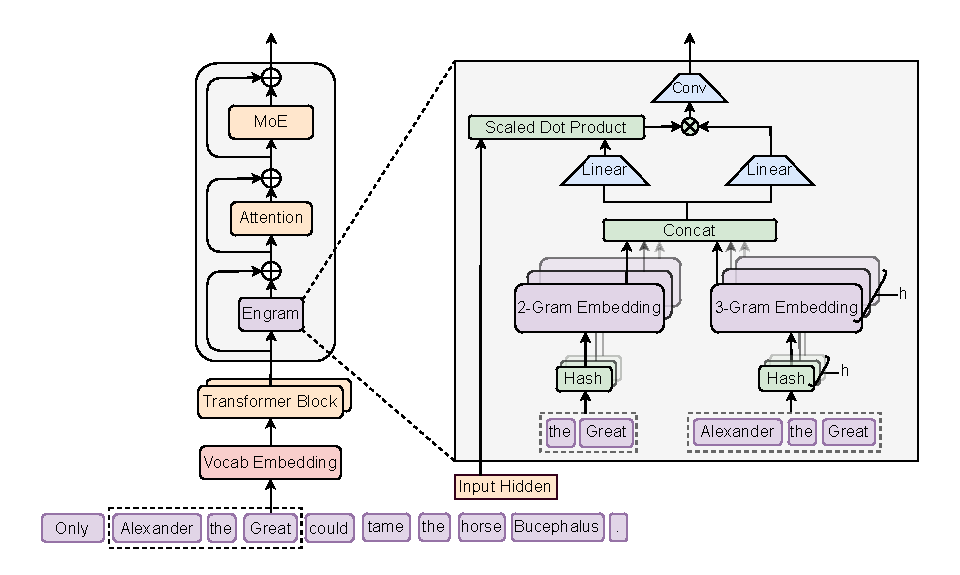
\includegraphics[width=.96\textwidth]{../papers/translations/engram/figures/engram_arch.pdf}
\caption{原文图1: Engram架构. 检索静态$N$-gram记忆,通过上下文感知门控与动态隐状态融合. 仅在特定层插入,将记忆与计算分离;标准输入embedding与输出投影不变. 图内Vocab Embedding为词表嵌入,Input Hidden为输入隐状态,Hash为哈希,Concat为拼接,Linear为线性投影,Scaled Dot Product为缩放点积,Conv为卷积,Attention为注意力,MoE为混合专家. 原示例完整为“Only Alexander the Great could tame the horse Bucephalus.”,意为“只有亚历山大大帝能驯服名为Bucephalus的马”;示意后缀“the Great”和“Alexander the Great”的2/3-gram查找.}\label{engram-fig-1}
\end{figure}

\subsection*{2.2 基于哈希$N$-gram的稀疏检索}\paperlabel{2.2}{engram-sec-2-2}
第一阶段把局部上下文映射成静态记忆项, 包括分词器压缩与确定性哈希检索.

\noindent\textbf{分词器压缩.}\label{engram-token-compression}
普通 $N$-gram 模型通常直接使用分词结果, 标准子词分词器却优先保证无损重建, 常给语义等价形式分配不同 ID, 如 \texttt{Apple} 与带前导空格的 \texttt{apple}\cite{engram-kudo2018sentencepiecesimplelanguageindependent,engram-li2023starcodersourceyou}. 为提高语义密度, 我们加入词表投影层. 预先计算满射 $\mathcal P:V\to V'$, 按正规化的文本等价关系, 包括 NFKC\cite{engram-UAX15-NFKC}、小写转换等, 把原始 token ID 合并成规范标识. 对 128k 分词器, 有效词表大小实际减少约 $23\%$, 例子见附录 C. 位置 $t$ 的原 ID $x_t$ 被映射为 $x'_t=\mathcal P(x_t)$, 并构成后缀 $N$-gram $g_{t,n}=(x'_{t-n+1},\ldots,x'_t)$.

\noindent\textbf{多头哈希.}\label{engram-multi-head-hash}
所有可能 $N$-gram 的组合空间无法直接参数化. 按既有方法\cite{engram-tito2017hash}, 我们采用哈希. 为减轻碰撞, 每个阶数 $n$ 使用 $K$ 个不同哈希头. 第 $k$ 个头以确定函数 $\phi_{n,k}$ 把压缩上下文映射为 embedding 表 $\mathbf E_{n,k}$ 的索引, 该表大小 $M_{n,k}$ 为素数:
\begin{equation}\label{engram-eq-1}
z_{t,n,k}\triangleq\phi_{n,k}(g_{t,n}),\qquad
\mathbf e_{t,n,k}=\mathbf E_{n,k}[z_{t,n,k}].
\end{equation}
实际的 $\phi_{n,k}$ 用轻量乘法--异或哈希实现. 最终记忆向量 $\mathbf e_t\in\R^{d_{\rm mem}}$ 拼接所有检索到的 embedding:
\begin{equation}\label{engram-eq-2}
\mathbf e_t\triangleq\mathop{\Vert}_{n=2}^{N}\mathop{\Vert}_{k=1}^{K}\mathbf e_{t,n,k}.
\end{equation}

\subsection*{2.3 上下文感知门控}\paperlabel{2.3}{engram-sec-2-3}
检索得到的 $\mathbf e_t$ 是与上下文无关的先验. 静态性质使它缺少上下文适应能力, 哈希碰撞或多义性也可能引入噪声\cite{engram-haber-poesio-2024-polysemy}. 为增强表达并消除歧义, 我们采用受注意力启发的上下文感知门控\cite{engram-vaswani2017attention,engram-bahdanau2014neural}. 当前隐状态 $\mathbf h_t$ 已通过先前注意力层聚合全局上下文, 被作为动态 Query; 记忆 $\mathbf e_t$ 同时用于 Key 与 Value 投影:
\begin{equation}\label{engram-eq-3}
\mathbf k_t=\mathbf W_K\mathbf e_t,\qquad\mathbf v_t=\mathbf W_V\mathbf e_t.
\end{equation}
$\mathbf W_K,\mathbf W_V$ 是可学习投影矩阵. 为保证梯度稳定\cite{engram-pmlr-v202-dehghani23a}, 计算标量门 $\alpha_t\in(0,1)$ 前, 对 Query 和 Key 使用 RMSNorm\cite{engram-zhang2019root}:
\begin{equation}\label{engram-eq-4}
\alpha_t=\sigma\left(\frac{\operatorname{RMSNorm}(\mathbf h_t)^\top
\operatorname{RMSNorm}(\mathbf k_t)}{\sqrt d}\right).
\end{equation}
门控输出为 $\tilde{\mathbf v}_t=\alpha_t\mathbf v_t$. 作者认为这一设计强制语义对齐: 若检索记忆与当前上下文冲突, 门值倾向零, 从而抑制噪声.

最后, 为扩大感受野并增强非线性, 引入短的逐通道因果卷积\cite{engram-gu2021efficiently,engram-peng2023rwkv}. 令门控值序列 $\tilde{\mathbf V}\in\R^{T\times d}$, 卷积核大小 $w=4$, 膨胀率 $\delta$ 取最大 $N$-gram 阶数, 激活为 SiLU\cite{engram-elfwing2018sigmoid}, 最终输出是
\begin{equation}\label{engram-eq-5}
\mathbf Y=\operatorname{SiLU}\left(\operatorname{Conv1D}
(\operatorname{RMSNorm}(\tilde{\mathbf V}))\right)+\tilde{\mathbf V}.
\end{equation}
Engram 通过残差接入骨干, $\mathbf H^{(\ell)}\leftarrow\mathbf H^{(\ell)}+\mathbf Y$, 随后仍进行标准 Attention 和 MoE. 关键是, 不在每层都使用 Engram; 放置位置需平衡建模效果与后文的系统延迟约束.

\subsection*{2.4 与多分支架构集成}\paperlabel{2.4}{engram-sec-2-4}
本工作不用标准单流连接\cite{engram-he2016deep}, 默认采用建模能力更强的多分支骨干\cite{engram-larsson2016fractalnet,engram-zhu2025hyperconnections,engram-xie2025mhcmanifoldconstrainedhyperconnections,engram-szegedy2015going}. 其特征是把残差流扩展成 $M$ 个并行分支, 由可学习连接权重调制信息流.

Engram 本身不依赖拓扑, 但适配多分支时, 需要优化结构以平衡效率和表达. 具体采用参数共享: 所有 $M$ 个分支共享同一稀疏 embedding 表及 Value 投影 $\mathbf W_V$, 使用 $M$ 个不同 Key 投影 $\{\mathbf W_K^{(m)}\}_{m=1}^M$, 从而允许分支特定门控. 对隐状态为 $\mathbf h_t^{(m)}$ 的第 $m$ 个分支,
\begin{equation}\label{engram-eq-6}
\alpha_t^{(m)}=\sigma\left(\frac{\operatorname{RMSNorm}(\mathbf h_t^{(m)})^\top
\operatorname{RMSNorm}(\mathbf W_K^{(m)}\mathbf e_t)}{\sqrt d}\right).
\end{equation}
独立门控调制共享值向量, $\mathbf u_t^{(m)}=\alpha_t^{(m)}(\mathbf W_V\mathbf e_t)$. 这样一个 $\mathbf W_V$ 与 $M$ 个 Key 投影可以融合为一次稠密 FP8 矩阵乘法, 提高现代 GPU 利用率. 未另说明时, 所有实验均使用这种与流形约束超连接(mHC, $M=4$)的集成\cite{engram-xie2025mhcmanifoldconstrainedhyperconnections}.

\subsection*{2.5 系统效率: 计算与记忆解耦}\paperlabel{2.5}{engram-sec-2-5}
参数扩展常受 GPU 高带宽显存(HBM)容量限制. MoE 基于运行时隐状态动态路由, Engram 则仅依赖输入 token ID 确定性检索, 因而自然分离参数存储与计算. 这种可预测性使训练、推断都能特别优化, 见图 \ref{engram-fig-2}.

\begin{figure}[htbp]
\centering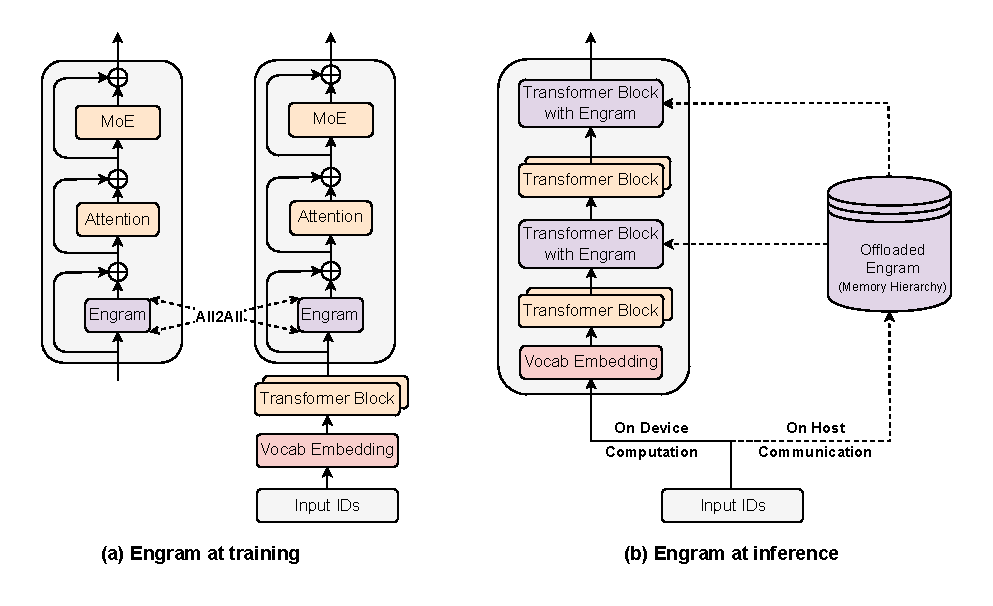
\includegraphics[width=.96\textwidth]{../papers/translations/engram/figures/engram_system.pdf}
\caption{原文图2: Engram系统实现. (a)训练时,大embedding表分片到GPU,用All-to-All跨设备读取激活行. (b)推断时,表卸载到主机内存,主机利用确定检索异步预取并传输embedding,让通信与先前Transformer模块计算重叠. 图内On Device Computation/On Host Communication分别为设备计算/主机通信,Input IDs为输入编号,Vocab Embedding为词表嵌入,Offloaded Engram为卸载的记忆表,Memory Hierarchy为存储层级,All2All为全互联通信,Transformer Block为Transformer模块.}\label{engram-fig-2}
\end{figure}

训练中, 我们用标准模型并行把大表分片到各 GPU. 前向以 All-to-All 收集激活行, 后向用它分发梯度, 让总记忆容量随加速器数量线性增长.

推断中, 确定性允许预取和重叠策略. 前向之前就知道记忆索引, 系统可以通过 PCIe 从充足的主机内存异步取 embedding. 为掩盖通信延迟, 将 Engram 放在骨干特定层, 借先前层计算作为缓冲, 避免 GPU 停顿. 这需要硬件与算法共同设计: 放得更深, 隐藏延迟的计算窗口更大; 但结构消融显示, 建模效果偏好尽早介入, 卸下局部模式重建. 因而最优位置同时受建模和延迟约束.

此外, 自然语言 $N$-gram 遵循 Zipf 分布\cite{engram-piantadosi2014zipf,engram-Chao1950HumanBA}, 少数模式占据大多数访问. 这支持多级缓存: 常用 embedding 放在 GPU HBM 或主机 DRAM 等较快层级, 罕见长尾放在 NVMe SSD 等慢而大容量介质. 作者认为这种分层可让 Engram 扩展到很大记忆容量, 而有效延迟影响很小.

\originalsection{3 扩展规律与稀疏分配}\paperlabel{3}{engram-sec-3}
条件记忆的 Engram 与条件计算的 MoE 专家在结构上互补. 本节研究这种双重结构的扩展性质及最优稀疏容量分配, 关注两个问题: 总参数和训练计算固定时, 容量如何分给专家与 embedding? 如果利用 Engram 的 $\mathcal O(1)$ 开销特征放宽或大幅扩展记忆预算, 单独 Engram 表现出怎样的扩展行为?

\begin{figure}[htbp]
\centering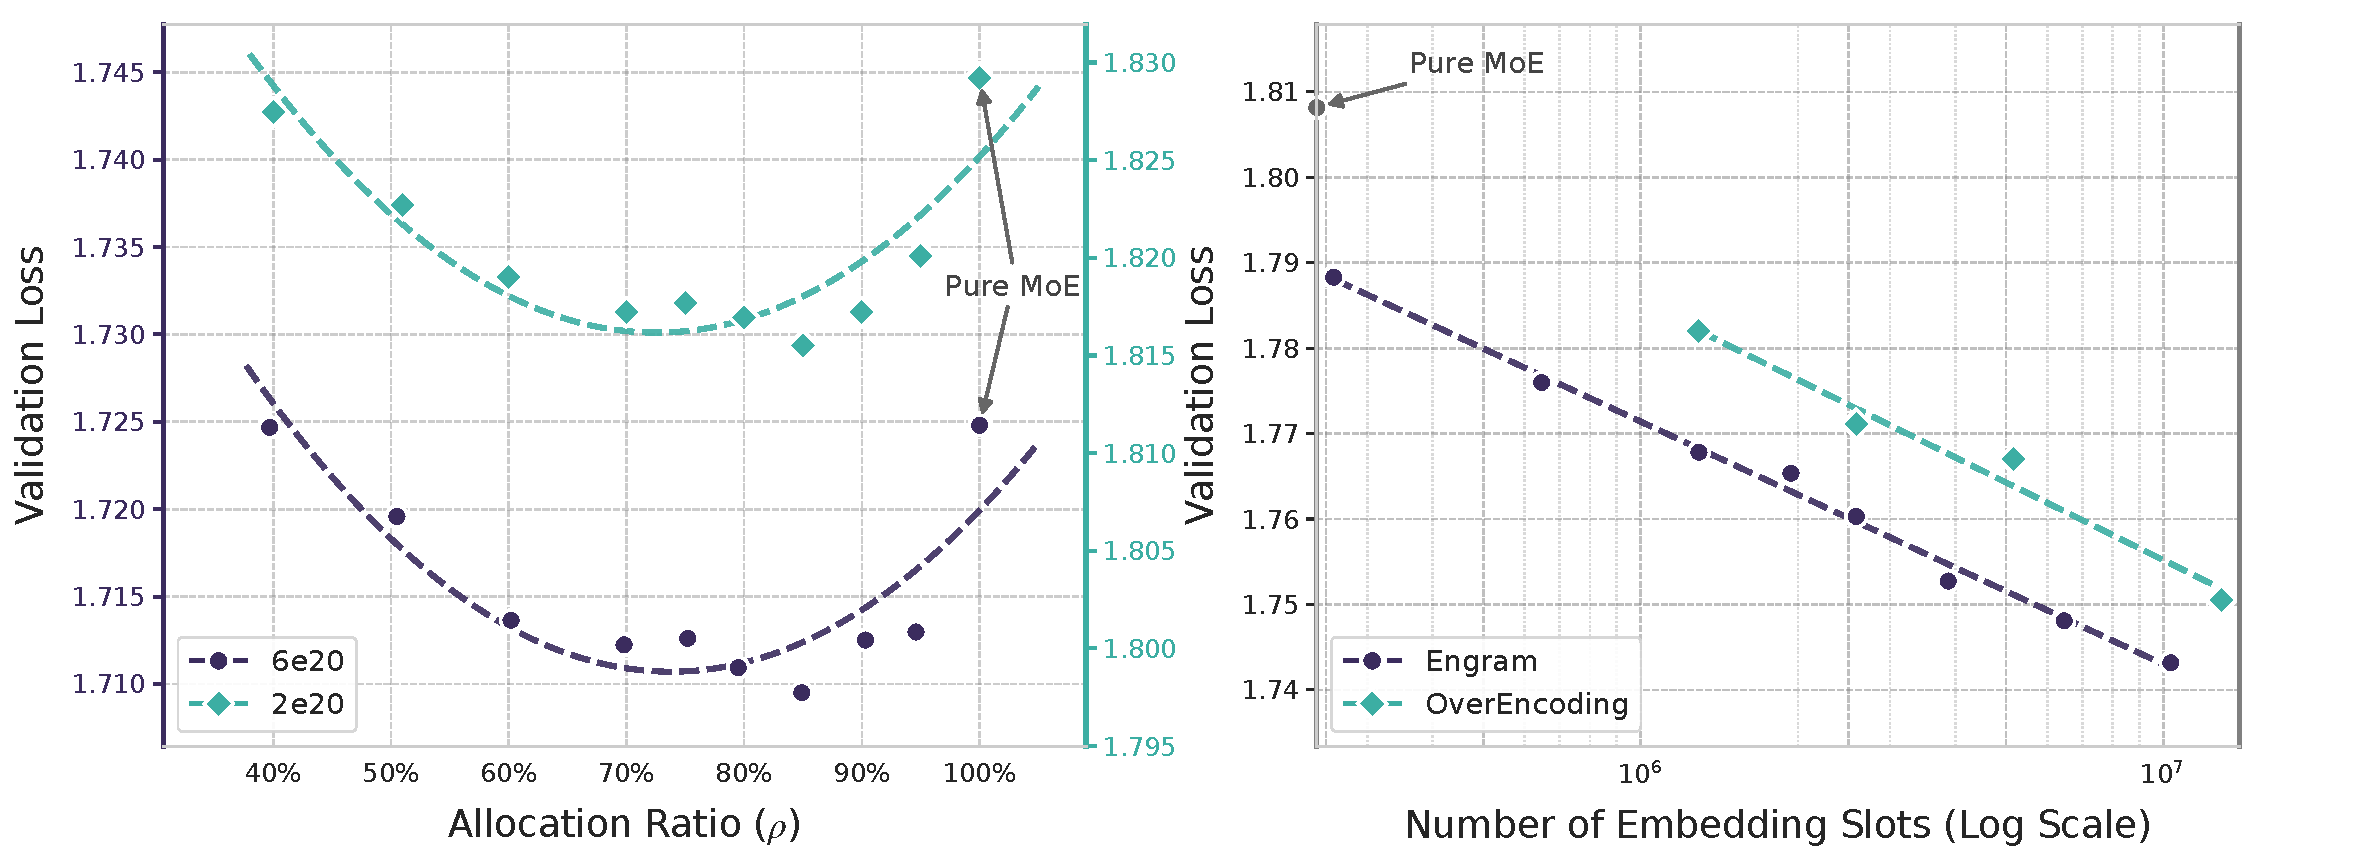
\includegraphics[width=.98\textwidth]{../papers/translations/engram/figures/scaling_law.pdf}
\caption{原文图3: 稀疏分配与Engram扩展. 左: 分配比例$\rho$对应验证损失,展示$2\times10^{20}$和$6\times10^{20}$ FLOPs预算,两者均为U形,混合分配优于纯MoE. 右: 所谓无限记忆设置,验证损失与embedding数量呈对数线性趋势. 图内Allocation Ratio为分配比例,Validation Loss为验证损失,Number of Embedding Slots (Log Scale)为记忆槽数(对数坐标),Pure MoE为纯MoE,OverEncoding为对照方法.}\label{engram-fig-3}
\end{figure}

\subsection*{3.1 MoE与Engram的最优分配比例}\paperlabel{3.1}{engram-sec-3-1}
\noindent\textbf{计算匹配形式化.}
用三项参数指标分析权衡. $P_{\rm tot}$ 是总可训练参数, 不含词表 embedding 和 LM head. $P_{\rm act}$ 是每个 token 的激活参数, 决定训练 FLOPs. $P_{\rm sparse}\triangleq P_{\rm tot}-P_{\rm act}$ 是不激活参数, 代表不增加计算即可扩模型的“免费”参数预算, 如未选专家或未检索 embedding.

每个 FLOPs 预算中固定 $P_{\rm tot}$ 和 $P_{\rm act}$, 使总参数和每 token FLOPs 相同. MoE 的 $P_{\rm act}$ 由 top-$k$ 专家决定, 其余专家进入 $P_{\rm sparse}$. Engram 每 token 只读取常数个槽, 因而扩槽数增加总参数, 不增加每 token FLOPs.

\noindent\textbf{分配比例.}
$\rho\in[0,1]$ 定义为不激活参数预算中分给 MoE 专家的比例:
\begin{equation}\label{engram-eq-7}
P_{\rm MoE}^{(\rm sparse)}=\rho P_{\rm sparse},\qquad
P_{\rm Engram}=(1-\rho)P_{\rm sparse}.
\end{equation}
$\rho=1$ 为纯 MoE, 全部不激活参数都是路由专家. $\rho<1$ 时减少路由专家, 把释放的参数分给 Engram 槽.

\noindent\textbf{实验协议.}
比较两项计算预算, 稀疏比 $P_{\rm tot}/P_{\rm act}\approx10$ 保持相同. $C=2\times10^{20}$ FLOPs 时, $P_{\rm tot}\approx5.7$B, $P_{\rm act}=568$M, $\rho=1$ 基线共106个专家. $C=6\times10^{20}$ FLOPs 时, $P_{\rm tot}\approx9.9$B, $P_{\rm act}=993$M, 基线共99个专家. 不同 $\rho$ 仅调整路由专家数和 Engram 槽数, 训练流程和优化超参数完全一致.

\noindent\textbf{结果与分析.}
图 \ref{engram-fig-3} 左侧显示, 验证损失与 $\rho$ 有一致的 U 形关系. 即使 MoE 分配减少到约 $40\%$, Engram 仍与纯 MoE 的 $100\%$ 分配性能相近; 5.7B模型共46个专家, 9.9B模型共43个专家. 纯 MoE 并非最优, 把稀疏预算约 $20\%$--$25\%$ 分给 Engram 时最好. 10B设置、$6\times10^{20}$ FLOPs 中, 损失由纯MoE的 $1.7248$ 降为接近 $\rho=80\%$ 最优点的 $1.7109$, 差为 $0.0139$.

两个规模的最优位置均约 $75\%$--$80\%$, 表明在已考察规模和固定稀疏度下偏好稳定. 作者认为 U 形关系确认两模块结构互补: MoE占主导时缺少静态模式专用记忆, 只能低效地用深度和计算重建; Engram占主导时失去条件计算容量, 损害动态上下文推理, 记忆不能替代计算.

\subsection*{3.2 无限记忆设置中的Engram}\paperlabel{3.2}{engram-sec-3-2}
前面固定总参数, 现在考察更激进的记忆扩展, 动机是存储与计算解耦.

\noindent\textbf{实验协议.}
固定约3B总参数、568M激活参数的 MoE 骨干, 训练100B token以确保收敛. 加 Engram 表, 槽数 $M$ 从 $2.58\times10^5$ 到 $1.0\times10^7$, 最多增加约13B参数. 对照为 OverEncoding\cite{engram-huang2025over}, 它把 $N$-gram embedding 与词表 embedding 平均融合. SCONE\cite{engram-yu2025scaling}虽也研究大embedding, 但主要着眼推断, 包含额外 f-gram 模块和训练FLOPs, 不符合本研究严格等计算条件.

\noindent\textbf{结果.}
图 \ref{engram-fig-3} 右侧显示槽数增加清楚而持续地改善验证损失. 在考察区间, 作者称曲线满足严格幂律, 在对数空间线性, 因而把 Engram 视为可预测的扩展旋钮: 更大记忆持续有收益, 无需额外计算. OverEncoding的直接平均也受益于大表, 但同一记忆预算下, Engram释放更大扩展潜力. 结合前述分配规律, 作者据此认为条件记忆是独立且可扩展的稀疏容量轴, 与MoE条件计算互补.

\originalsection{4 大规模预训练}\paperlabel{4}{engram-sec-4}
使用提出的架构与经验分配规律, 我们训练多十亿参数模型, 检验真实语言模型预训练中的效用. 四个模型为 Dense-4B(总参数4.1B)、MoE-27B(26.7B)、Engram-27B(26.7B)与Engram-40B(39.5B). 全部使用相同数据课程, 即同样的token预算和顺序, 激活参数数目严格匹配.

\subsection*{4.1 实验设置}\paperlabel{4.1}{engram-sec-4-1}
\noindent\textbf{训练数据与模型配置.}
所有模型在262B token语料上预训练, 使用DeepSeek-V3\cite{engram-liu2024deepseek}的128k词表分词器. 为控制比较, 除明确例外外采用一致默认配置: 30个Transformer模块, 隐层2560. 各模块含32头多头潜在注意力(MLA)\cite{engram-deepseekai2024deepseekv2strongeconomicalefficient}, 以扩张率4的mHC\cite{engram-xie2025mhcmanifoldconstrainedhyperconnections}连接FFN. 全部使用Muon\cite{engram-jordan2024muon,engram-liu2025muon}优化, 详细超参数见附录A. 四种配置如下:
\begin{itemize}
\item Dense-4B为基线, 每个模块使用标准稠密FFN.
\item MoE-27B以DeepSeekMoE\cite{engram-dai2024deepseekmoe}替代稠密FFN, 含72个路由专家与2个共享专家, 每token选择top-$k=6$路由专家. 总参数26.7B, 激活参数与Dense-4B相同.
\item Engram-27B严格从MoE-27B得到: 路由专家72减为55, 释放参数给5.7B embedding模块, $\rho=74.3\%$, 总参数仍26.7B. Engram放在第2和15层, 最大$N$-gram为3, 头数8, 维度1280. embedding参数以Adam\cite{engram-kingma2014adam}更新, 学习率是基础值的5倍, 无权重衰减. 卷积参数零初始化, 作者称由此在训练开始严格保持恒等映射.
\item Engram-40B保持相同骨干和计算预算, 稀疏embedding扩至18.5B, 总参数39.5B, 用于研究Engram扩展性质.
\end{itemize}

\noindent\textbf{评价协议.}
评价覆盖语言建模、知识、推理、阅读理解、代码和数学, 各基准使用标准提示协议与指标.
\begin{itemize}
\item 语言建模报告The Pile\cite{engram-gao2020pile}测试损失, 以及从训练同分布抽取的验证集损失.
\item 知识与推理包括MMLU\cite{engram-hendrycks2020measuring}、MMLU-Redux\cite{engram-gema2025we}、MMLU-Pro\cite{engram-wang2024mmlu}、CMMLU\cite{engram-li2024cmmlu}、C-Eval\cite{engram-huang2023c}、AGIEval\cite{engram-zhong2024agieval}、ARC-Easy/Challenge\cite{engram-clark2018think}、TriviaQA\cite{engram-joshi2017triviaqa}、内部TriviaQA-ZH、PopQA\cite{engram-mallen2023not}、CCPM\cite{engram-li2021ccpm}、BBH\cite{engram-suzgun2023challenging}、HellaSwag\cite{engram-zellers2019hellaswag}、PIQA\cite{engram-bisk2020piqa}、WinoGrande\cite{engram-sakaguchi2021winogrande}.
\item 阅读理解包括DROP\cite{engram-dua2019drop}、RACE的Middle/High\cite{engram-lai2017race}以及C3\cite{engram-sun2020investigating}.
\item 代码与数学包括HumanEval\cite{engram-chen2021evaluatinglargelanguagemodels}、MBPP\cite{engram-austin2021program}、CruxEval\cite{engram-gu2024cruxeval}、GSM8K\cite{engram-cobbe2021training}、MGSM\cite{engram-shi2022language}与MATH\cite{engram-hendrycks2021measuring}.
\end{itemize}

\begingroup\setlength{\tabcolsep}{3pt}
\begin{longtable}{p{.32\textwidth}lrrrr}
\caption{原文表1: 稠密、MoE与Engram模型的预训练比较. 全部训练262B token,激活参数均为3.8B. Engram-27B将路由专家72减为55,换成5.7B参数的Engram记忆,与MoE-27B总参数相同. Engram-40B把记忆增到18.5B,激活预算不变. 完整末段训练曲线见附录B. EM为精确匹配,Pass@1为一次生成通过率.}\label{engram-tab-1}\\
\toprule
 基准(指标) & 示例数 & \shortstack{Dense\\4B} & \shortstack{MoE\\27B} & \shortstack{Engram\\27B} & \shortstack{Engram\\40B} \\
\midrule
 总参数 &  & 4.1B & 26.7B & 26.7B & 39.5B \\
 激活参数(不含词嵌入) &  & 3.8B & 3.8B & 3.8B & 3.8B \\
 训练token &  & 262B & 262B & 262B &  262B \\
 专家(共享+路由,top-$k$) &  & - & $2+72$ (top-6) & $2+55$ (top-6) & $2+55$ (top-6) \\
 Engram参数 &  & - & - & 5.7B & 18.5B \\
 \midrule
\multicolumn{6}{c}{语言建模}\\
Pile {(损失)} & - & 2.091 & 1.960 & \textbf{1.950} & 1.942 \\
 验证集 {(损失)} & - & 1.768 & 1.634 & \textbf{1.622} & 1.610 \\
 \midrule
\multicolumn{6}{c}{知识与推理}\\
MMLU {(准确率)} & 5-shot & 48.6 & 57.4 & \textbf{60.4} &  60.6 \\
 MMLU-Redux {(准确率)} & 5-shot & 50.7 & 60.6 & \textbf{64.0} & 64.5 \\
 MMLU-Pro {(准确率)} & 5-shot & 21.1 & 28.3 & \textbf{30.1} & 31.3  \\
 CMMLU {(准确率)} & 5-shot & 47.9 & 57.9 & \textbf{61.9} &  63.4 \\
 C-Eval {(准确率)} & 5-shot & 46.9 & 58.0 & \textbf{62.7} & 63.3 \\
 AGIEval {(准确率)} & 0-shot & 29.1 & 38.6 & \textbf{41.8} & 45.9 \\
 ARC-Easy {(准确率)} & 25-shot & 76.8 & 86.5 & \textbf{89.0} & 90.1 \\
 ARC-Challenge {(准确率)} & 25-shot & 59.3 & 70.1 & \textbf{73.8} &  76.4 \\
 TriviaQA {(EM)} & 5-shot & 33.0 & 48.8 & \textbf{50.7} & 51.8 \\
 TriviaQA-ZH {(EM)} & 5-shot & 62.8 & 74.8 & \textbf{76.3} & 77.9 \\
 PopQA {(EM)} & 15-shot & 15.1 & 19.2 & \textbf{19.4} & 21.2 \\
 CCPM {(准确率)} & 0-shot & 72.2 & 79.6 & \textbf{87.1} &  87.7 \\
 BBH {(EM)} & 3-shot & 42.8 & 50.9 & \textbf{55.9} &  57.5 \\
 HellaSwag {(准确率)} & 0-shot & 64.3 & 71.8 & \textbf{72.7} & 73.1 \\
 PIQA {(准确率)} & 0-shot & 63.8 & 71.9 & \textbf{73.5} &  76.5 \\
 WinoGrande {(准确率)} & 5-shot & 64.0 & 67.6 & \textbf{67.8} &  68.1 \\
 \midrule
\multicolumn{6}{c}{阅读理解}\\
DROP {(F1)} & 1-shot & 41.6 & 55.7 & \textbf{59.0} & 60.7 \\
 RACE-Middle {(准确率)} & 5-shot & 72.4 & 80.9 & \textbf{82.8} & 83.3 \\
 RACE-High {(准确率)} & 5-shot & 66.0 & 75.4 & \textbf{78.2} & 79.2 \\
 C3 {(准确率)} & 0-shot & 57.7 & 60.1 & \textbf{63.6} &  61.8 \\
 \midrule
\multicolumn{6}{c}{代码与数学}\\
HumanEval {(Pass@1)} & 0-shot & 26.8 & 37.8 & \textbf{40.8} & 38.4  \\
 MBPP {(Pass@1)} & 3-shot & 35.4 & 46.6 & \textbf{48.2} & 46.2 \\
 CruxEval-i {(EM)} & 0-shot &27.6&30.7 & \textbf{32.2} & 36.2 \\
 CruxEval-o {(EM)} & 0-shot &28.7&34.1 & \textbf{35.0} & 35.3 \\
 GSM8K {(EM)} & 8-shot & 35.5 & 58.4 & \textbf{60.6} & 62.6 \\
 MGSM {(EM)} & 8-shot & 27.0 & 46.8 & \textbf{49.4} &  52.4 \\
 MATH {(EM)} & 4-shot & 15.2 & 28.3 & \textbf{30.7} & 30.6 \\
\bottomrule
\end{longtable}
\endgroup


\subsection*{4.2 实验结果}\paperlabel{4.2}{engram-sec-4-2}
表 \ref{engram-tab-1} 汇总结果. 与既有文献\cite{engram-shazeer2017outrageously,engram-he2024mixture,engram-borgeaud2022improving}一致, 稀疏架构比稠密架构有更好的扩展规律. 同训练计算预算下, MoE-27B和Engram-27B/40B三种稀疏模型在全部基准显著优于等FLOPs的Dense-4B.

更重要的是, Engram-27B持续优于等参数、等FLOPs的MoE-27B. 收益不限于知识密集任务, 如本节报告MMLU $+3.0$, MMLU-Pro $+1.8$, CMMLU $+4.0$. 一般推理也有BBH $+5.0$, ARC-Challenge $+3.7$, DROP $+3.3$; 代码与数学有HumanEval $+3.0$, MBPP $+1.6$, GSM8K $+2.2$, MATH $+2.4$. 为降低基准噪声影响、展示训练动态, 附录B给出预训练完整基准轨迹. 这些结果支持作者假说: 专用知识查找原语能改善表征效率, 超过把全部稀疏预算给条件计算的方案.

Engram-40B进一步降低预训练损失, 改善大多数基准, 但并非每项任务严格优于27B. 作者推测原因是训练不足: 40B与基线的训练损失差在训练末期仍扩大, 暗示当前token预算尚未充分发挥新增记忆容量.

\originalsection{5 长上下文训练}\paperlabel{5}{engram-sec-5}
Engram把局部依赖建模交给静态查找, 为全局上下文保留注意力容量. 本节通过长上下文扩展训练\cite{engram-gao2025train,engram-peng2023yarn}检验这一结构优势, 尝试将架构贡献与基础模型能力分离, 报告长程检索和推理收益.

\subsection*{5.1 实验设置}\paperlabel{5.1}{engram-sec-5-1}
\noindent\textbf{训练细节.}
采用DeepSeek-V3\cite{engram-liu2024deepseek}的上下文扩展策略. 预训练后使用YaRN\cite{engram-peng2023yarn}, 在32768-token上下文阶段训练5000步, 使用30B高质量长上下文token. 超参数为$s=10$, $\alpha=1$, $\beta=32$, 缩放因子$f=0.707$.

\noindent\textbf{模型配置.}
四种模型的上下文扩展比较包括MoE-27B和Engram-27B的50k最终预训练检查点, 以及Engram-27B的41k和46k中间检查点. 初始化阶段不同, 但扩展训练协议完全相同. 特别选46k, 因为其预训练损失等于完整训练MoE-27B的50k, 构成“Iso-Loss”控制. 作者据此认为, 扩展后的差异可归于架构, 而不是起始模型质量.

\noindent\textbf{评价基准.}
LongPPL\cite{engram-fangwrong}包含长书籍、研究论文、代码库和长思维链轨迹四类. RULER\cite{engram-hsiehruler}包含14个子集, 汇成8类: 大海捞针(NIAH)的单针(S)、多键(MK)、多值(MV)、多查询(MQ), 多跳变量跟踪(VT)、常见词提取(CWE)、高频词提取(FWE)和问答(QA).

\begin{table}[htbp]
\centering\begingroup\setlength{\tabcolsep}{3pt}
\caption{原文表2: 长上下文性能,32k长度. 译稿把原模型行与指标列转置,每个数据单元保留. 括号为扩展训练前的预训练步数及损失. LongPPL越低越好,RULER准确率越高越好;粗体和下划线保留作者标记.}\label{engram-tab-2}
\begin{tabular}{lrrrr}\toprule
指标 & \shortstack{MoE-27B\\(50k,1.63)} & \shortstack{Engram-27B\\(41k,1.66)} & \shortstack{Engram-27B\\(46k,1.63)} & \shortstack{Engram-27B\\(50k,1.62)} \\
\midrule
LongPPL:书籍 & 4.38 & 4.37 & \underline{4.19} & \textbf{4.14} \\
LongPPL:论文 & 2.91 & 2.92 & \underline{2.84} & \textbf{2.82} \\
LongPPL:代码 & 2.49 & 2.50 & \underline{2.45} & \textbf{2.44} \\
LongPPL:长思维链 & 14.16 & 14.26 & \underline{13.59} & \textbf{13.41} \\
RULER:S & \textbf{100.0} & \underline{99.6} & 97.6 & 99.3 \\
RULER:MK & 88.0 & 88.3 & \underline{89.0} & \textbf{89.3} \\
RULER:MV & 92.7 & 93.0 & \underline{95.5} & \textbf{96.5} \\
RULER:MQ & 84.2 & 89.5 & \textbf{97.0} & \textbf{97.0} \\
RULER:VT & 77.0 & 83.2 & \underline{87.2} & \textbf{89.0} \\
RULER:CWE & \underline{4.5} & 3.8 & 4.3 & \textbf{5.9} \\
RULER:FWE & 73.0 & 99.6 & \underline{98.6} & \textbf{99.3} \\
RULER:QA & 34.5 & \textbf{44.0} & 37.5 & \underline{40.5} \\
\bottomrule
\end{tabular}
\endgroup
\end{table}


\subsection*{5.2 实验结果}\paperlabel{5.2}{engram-sec-5-2}
结果见表 \ref{engram-tab-2}. 分析分两步, 先分离基础模型能力与架构的影响, 再进行控制比较.

\noindent\textbf{1. 不只由注意力机制决定的长上下文能力.}
注意力和位置编码提供上下文处理结构基础\cite{engram-su2023roformerenhancedtransformerrotary,engram-press2021train,engram-yang2025path,engram-xiao2023efficient}, 但结果表明长上下文性能不只由架构先验决定. 原文称, Engram由41k到50k的轨迹显示, 在架构相同、上下文扩展计算预算固定时, 预训练推进带来单调改善. 作者认为这提示长上下文与一般建模能力内在相连, 因而严格比较应对齐基础模型损失, 不只对齐训练步数.

\noindent\textbf{2. 控制设置中的架构优势.}
按上述原则, 比较Engram与MoE.
\begin{itemize}
\item 等损失设置: Engram-27B的46k与MoE-27B的50k预训练损失相同. 作者称它严格分离架构效率, Engram在复杂检索任务显著更好, 如多查询NIAH $97.0$ 对 $84.2$, VT $87.2$ 对 $77.0$.
\item 等FLOPs设置: 两者均50k, Engram进一步扩大差距. 原文称它取得全面最高性能.
\item 极端设置: Engram仅41k, 约82\%预训练计算, 仍与完整MoE有竞争力. 作者称它匹配LongPPL并在RULER超过基线, 展示架构固有优势.
\end{itemize}
原表图注还概括两点: 41k用82\%预训练FLOPs, LongPPL匹配而RULER准确率明显更高; 46k等预训练损失和50k等预训练FLOPs时, Engram在所有指标显著更好. 这些为作者概括, 完整数值均在表 \ref{engram-tab-2} 保留.

\originalsection{6 分析}\paperlabel{6}{engram-sec-6}
本节研究Engram内部机制, 包括有效深度、核心模块与参数敏感性, 还评价卸载推断吞吐, 最后给出门控可视化案例.

\subsection*{6.1 Engram在功能上是否等于增加模型深度?}\paperlabel{6.1}{engram-sec-6-1}
当前LLM缺少专用知识查找原语, 依赖计算模拟记忆回想. 表 \ref{engram-tab-3} 显示, 为识别“Diana, Princess of Wales”, LLM使用多个注意力和FFN层逐步组合特征\cite{engram-li2025echoesbertmodernlanguage,engram-ghandeharioun2024patchscopes,engram-DBLP:conf/coling/JinYHZWH0MMDYDZ25}, 理论上这可以用知识查找来识别. 我们因此提出假说: 显式查找免去早期特征组合, 在效果上模拟深度增加. 用LogitLens\cite{engram-nostalgebraist2020logitlens,engram-belrose2023eliciting}与中心化核对齐(CKA)\cite{engram-kornblith2019similarity,engram-davari2022reliability}检验.

\begin{table}[htbp]
\centering\begingroup\setlength{\tabcolsep}{3pt}
\caption{原文表3: 从Ghandeharioun等的Patchscopes\cite{engram-ghandeharioun2024patchscopes}转引的实体解析例子. 多层注意力与FFN逐渐构建“Diana, Princess of Wales”的表示. 中列是PatchScope对最后token“Wales”的自动生成文本,下列保留英文并附中文翻译;右列为原作者人工解释. 该第三方论文另经官方arXiv许可核对为CC BY4.0,作者为Asma Ghandeharioun、Avi Caciularu、Adam Pearce、Lucas Dixon和Mor Geva,见\url{https://proceedings.mlr.press/v235/ghandeharioun24a.html}.}\label{engram-tab-3}
\begin{tabular}{rp{.54\textwidth}p{.33\textwidth}}\toprule
层 & 潜状态翻译 & 原作者解释\\\midrule
1--2 & : Country in the United Kingdom\par : 位于英国的国家 & Wales(威尔士)\\
3 & : Country in Europe\par : 位于欧洲的国家 & Wales(威尔士)\\
4 & : Title held by female sovereigns in their own right or by queens consort\par : 女性在位君主或王后拥有的头衔 & Princess of Wales(威尔士王妃), 不特指个人\\
5 & : Title given to the wife of the Prince of Wales (and later King)\par : 授予威尔士亲王(后来成为国王)妻子的头衔 & Princess of Wales(威尔士王妃), 不特指个人\\
6 & : Diana, Princess of Wales (1961-1997), the first wife of Prince Charles, Prince of Wales, who was famous for her beauty and humanitarian work\par : 戴安娜, 威尔士王妃(1961--1997), 威尔士亲王查尔斯的第一任妻子, 以美貌和人道主义工作闻名 & Diana, Princess of Wales(戴安娜, 威尔士王妃)\\\bottomrule
\end{tabular}\endgroup
\end{table}

\noindent\textbf{预测收敛加快.}\label{engram-logitlens}
先用LogitLens分析预测跨层演化. 每层隐状态用最终LM Head投影, 计算中间输出分布与模型最终输出分布的KL散度\cite{engram-kullback1951information}. 这量化潜表示离“预测就绪”有多近\cite{engram-csordas2025language,engram-belrose2023eliciting}. 图 \ref{engram-fig-4}(a)显示, 两种Engram相较MoE都有系统性更小的KL, 早期模块差距最明显. 作者认为更陡下降说明特征组合更快, 与显式访问知识减少计算步数、较早得到高置信度有效预测的假说相符.

\noindent\textbf{表征对齐与有效深度.}\label{engram-cka}
为考察Engram浅层是否在语义上对应更深的基线层, 使用广泛用于表征结构比较的CKA\cite{engram-kornblith2019similarity,engram-kriegeskorte2008representational}. 给定两组表示$X,Y$, 如不同模型或层的激活,
\begin{equation}\label{engram-eq-8}
\operatorname{CKA}(K,L)=\frac{\operatorname{HSIC}(K,L)}{
\sqrt{\operatorname{HSIC}(K,K)\operatorname{HSIC}(L,L)}}.
\end{equation}
$K=XX^\top$, $L=YY^\top$是线性核Gram矩阵, HSIC为Hilbert--Schmidt独立性准则\cite{engram-gretton2005measuring}. 使用小批次实现及无偏HSIC估计\cite{engram-davari2022reliability}, 在Few-NERD\cite{engram-ding2021few}上取命名实体最后token隐状态.

先计算逐层成对CKA矩阵$S\in[0,1]^{L\times L}$, $L$为层数. 再用每个Engram层$j$最相似的top-$k$个MoE层的加权质心定义软对齐指标:
\begin{equation}\label{engram-eq-9}
a_j=\frac{\sum_{i\in\mathcal I_j}S_{i,j}i}{\sum_{i\in\mathcal I_j}S_{i,j}},
\qquad\mathcal I_j=\mathop{\mathrm{argtop}k}_{i}(S_{i,j}).
\end{equation}
$S_{i,j}$为MoE层$i$与Engram层$j$的相似度; $a_j$代理该Engram层对应的“有效MoE深度”. top-$k$过滤取$k=5$, 减轻低相似度噪声.

图 \ref{engram-fig-4}(b,c)将软对齐曲线(白虚线)叠在相似度热图上. 高相似对角线明显上移, 很多层满足$a_j>j$. 例如Engram-27B第5层最接近MoE约第12层的表示. 这种持续的非对角偏移与LogitLens一致, 作者据此称Engram较早形成更深表示, 并验证核心假说: 显式查找绕过早期特征组合, 在功能上等于提高有效深度.

\begin{figure}[htbp]
\centering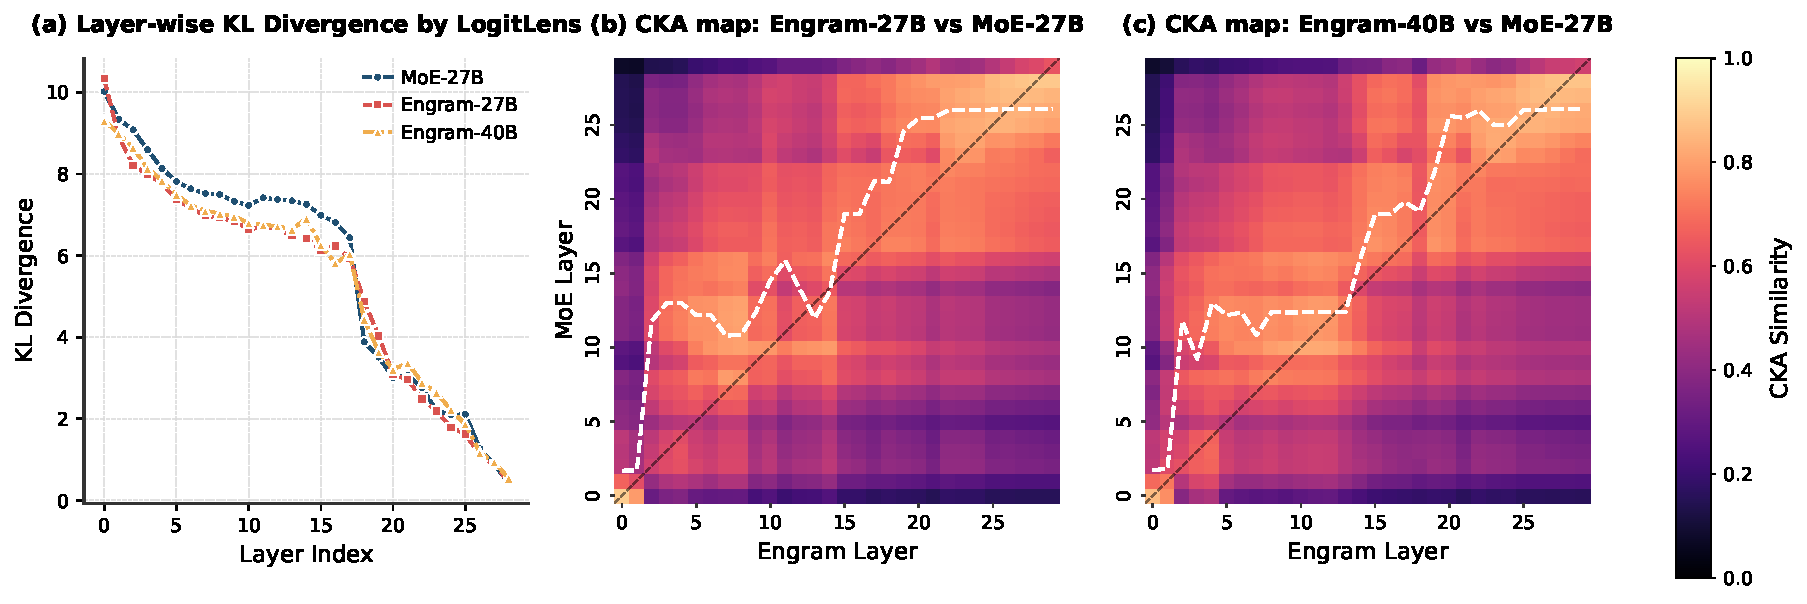
\includegraphics[width=\textwidth]{../papers/translations/engram/figures/logitlens_and_cka.pdf}
\caption{原文图4: 表征对齐与收敛速度. (a)逐层LogitLens KL散度,早期层较低散度表示预测较快趋近最终分布. (b,c)CKA相似度热图,高相似区域上移;作者把它解释为Engram浅层相当于MoE深层,从而增加有效深度. 图内Layer Index/Engram Layer/MoE Layer为层编号/Engram层/MoE层,KL Divergence为KL散度,CKA Similarity为CKA相似度. 图注原文有“=Engram”多余等号,译稿在排版上去掉这一明显标点错误.}\label{engram-fig-4}
\end{figure}

\subsection*{6.2 结构消融与层敏感性}\paperlabel{6.2}{engram-sec-6-2}
在受控设置中检验各设计. 未说明例外时, 骨干是12层3B MoE, 激活参数0.56B, 训练100B token. 图 \ref{engram-fig-5} 报告验证损失, 橙虚线是MoE基线$1.808$.

\noindent\textbf{参考配置.}
添加固定1.6B Engram记忆, 使用$\{2,3\}$-gram, 插入第2和6层, 验证损失$1.768$, 相比MoE改善$0.04$. 后面所有结构消融相对这个参考模型定义.

\noindent\textbf{记忆放在哪里?}
固定1.6B预算, 合并成单个模块, 扫描第1--12层. 这暴露放置权衡: 早插入能在骨干花费计算深度之前卸掉局部模式重建, 对应自然层级处理\cite{engram-tenney2019bert,engram-ghandeharioun2024patchscopes,engram-li2025echoesbertmodernlanguage,engram-DBLP:conf/coling/JinYHZWH0MMDYDZ25}. 但早期隐状态尚未经注意力充分聚合全局上下文, 并行分支也缺少精细调制所需的表征分化\cite{engram-xie2025mhcmanifoldconstrainedhyperconnections,engram-zhu2025hyperconnections}, 门控精度因此受影响. 最优位置需平衡尽早卸载静态模式与稍晚更强的上下文Query.

单模块最好为第2层, 损失$1.770$, 优于第1层, 更深则变差. 作者据此认为一轮注意力已给门控提供有意义的上下文, 同时足够早, 能替代底层局部聚合. 把同一1.6B记忆通过缩小$d_{\rm mem}$分成两个模块, 放第2和6层, 更好地达到$1.768$. 分层结合早期介入与后期丰富上下文门控, 还方便利用系统记忆层级.

\noindent\textbf{哪些组件重要?}
从参考配置逐个去掉设计, 记忆参数预算固定. 最重要的三项是多分支骨干中的分支特定融合、上下文门控、分词器压缩. 去掉任一项使损失回退最大. “w/o multi branch”仍保留mHC骨干, 只把分支门控改成在预映射$\mathcal H^{\rm pre}$之后对隐状态做一次Engram融合\cite{engram-xie2025mhcmanifoldconstrainedhyperconnections}.

其他变化较小: 去掉轻量逐通道卷积仅略微变差; 固定1.6B预算下分容量给4-gram略次优, 可能挤占更频繁的2/3-gram容量, 但不排除大记忆时高阶有益.

\begin{figure}[htbp]
\centering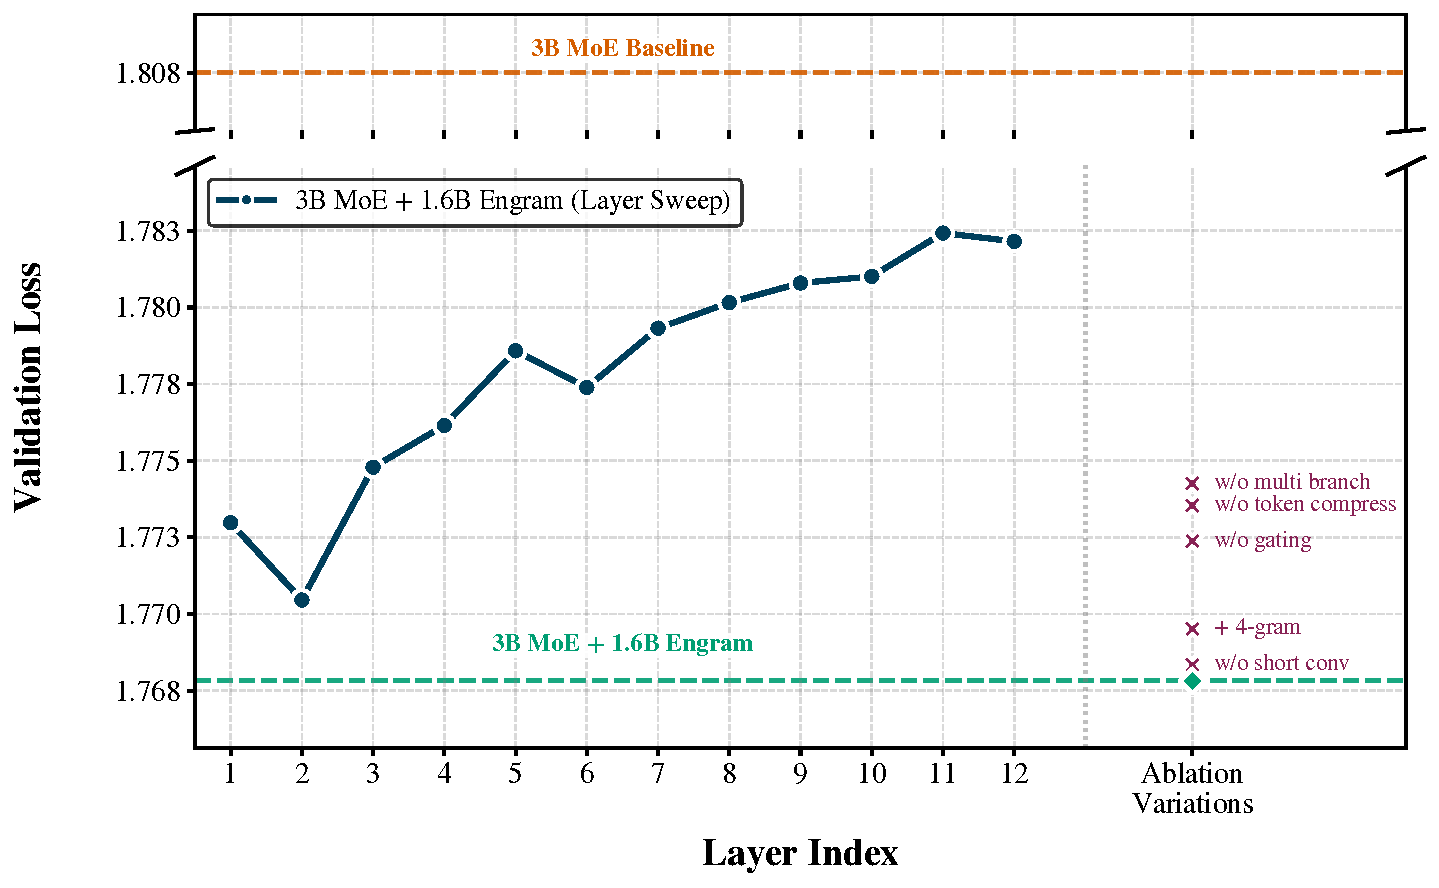
\includegraphics[width=.86\textwidth]{../papers/translations/engram/figures/arch_ablation.pdf}
\caption{原文图5: 架构消融. 深蓝曲线扫描单模块插入层,早期第2层最好,更深变差;右侧标记去掉参考配置子模块,显示多分支、压缩、门控的重要性. 图内Layer Index为层编号,Validation Loss为验证损失,Layer Sweep为逐层扫描,Ablation Variations为消融变体;w/o gating/w/o multi branch/w/o token compress/w/o short conv分别为无门控/无分支门控/无分词器压缩/无短卷积,+4-gram为加入4-gram.}\label{engram-fig-5}
\end{figure}

\subsection*{6.3 敏感性分析}\paperlabel{6.3}{engram-sec-6-3}
为刻画功能贡献, 推断时完全抑制稀疏embedding输出, 骨干不变. 关键是这种事后消融造成训练--推断不一致, 可能在混合复杂能力任务中引入噪声. 因而优先考察敏感谱两端的事实知识与阅读理解, 它们在此压力测试下信噪比最高.

图 \ref{engram-fig-6} 显示两类明显分化. 事实知识保留原性能的29\%--44\%, 如TriviaQA仅29\%, 作者据此称Engram是参数知识的主要仓库. 阅读理解保留81\%--93\%, 如C3为93\%, 表明有上下文依据的任务主要依赖骨干注意力而非Engram.
\begin{figure}[htbp]
\centering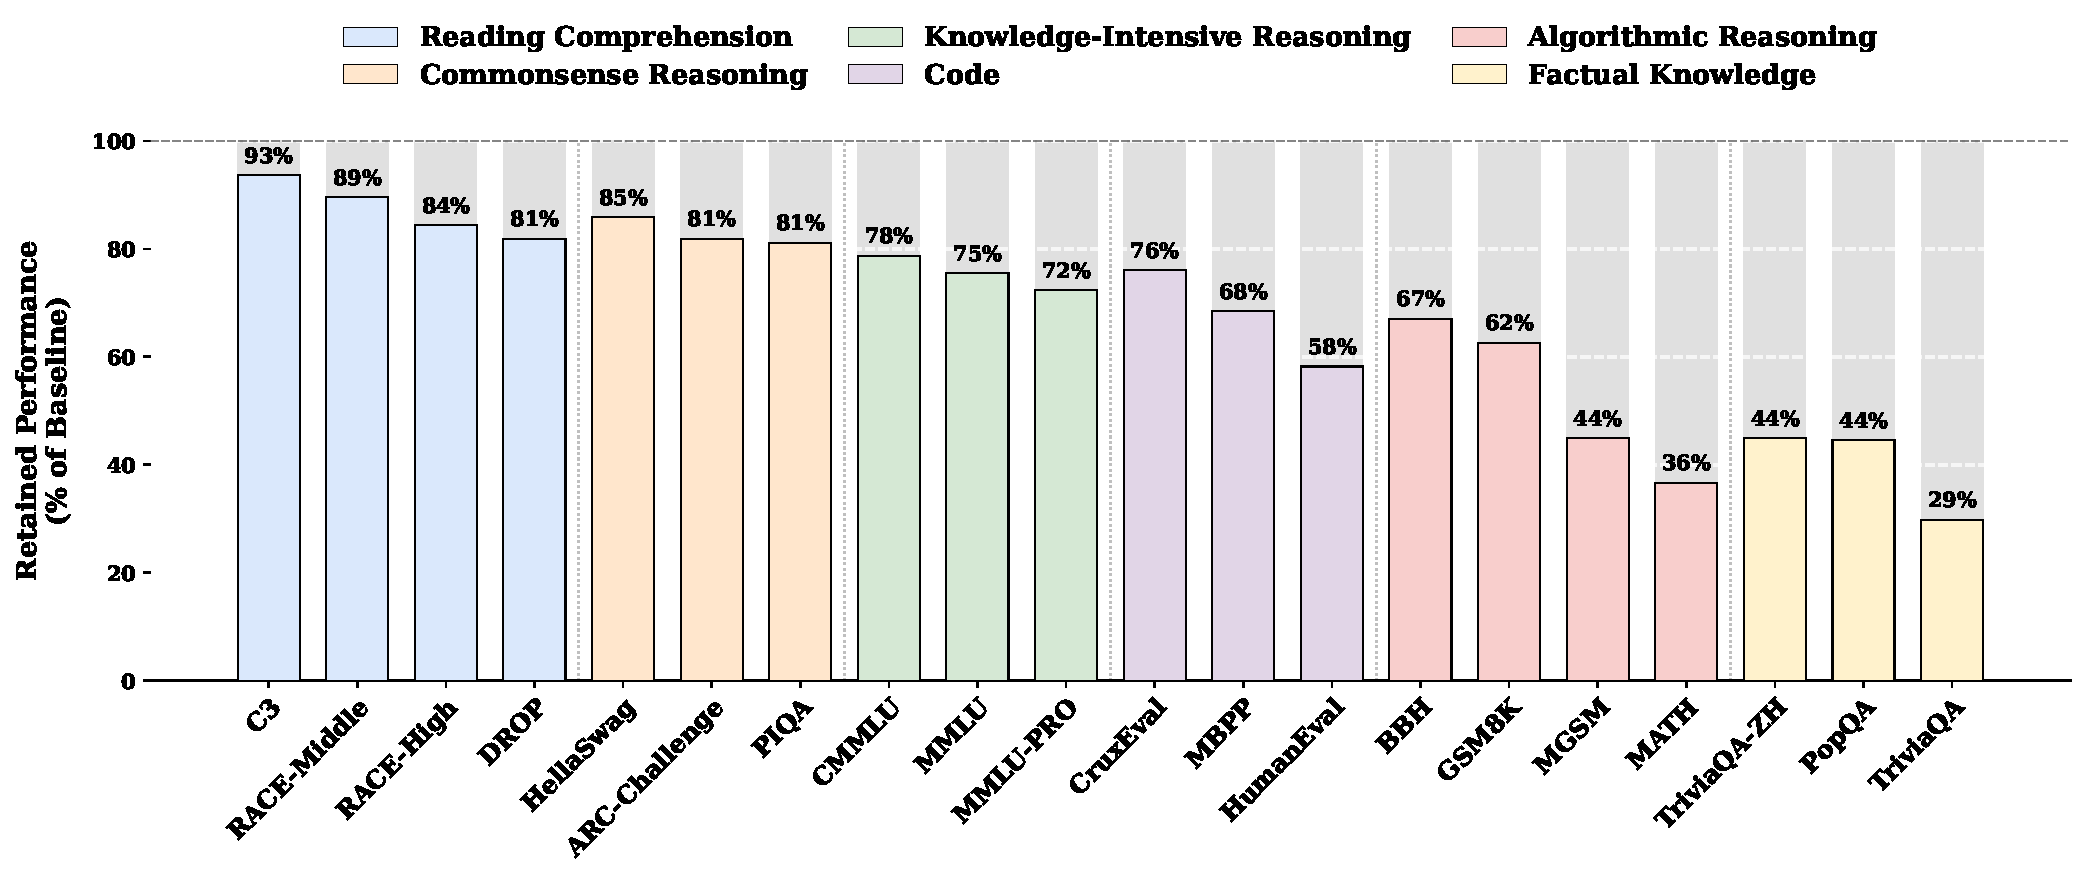
\includegraphics[width=.96\textwidth]{../papers/translations/engram/figures/sensitivity_analysis.pdf}
\caption{原文图6: 抑制Engram后的性能保留比例. 事实知识更依赖记忆模块,阅读理解更多由骨干保留. Retained Performance (\% of Baseline)为原性能保留百分比,不等于绝对准确率. 类别Reading Comprehension/Common Sense Reasoning/Knowledge-Intensive Reasoning/Code/Algorithmic Reasoning/Factual Knowledge分别为阅读理解/常识推理/知识密集推理/代码/算法推理/事实知识. 基准名与各百分比原样保留.}\label{engram-fig-6}
\end{figure}

\subsection*{6.4 系统效率}\paperlabel{6.4}{engram-sec-6-4}
相比按路由的MoE, Engram用显式静态哈希ID寻址稀疏激活. token序列已知时, 下一次查找索引确定, 可以在对应层执行前计算.

\noindent\textbf{实验设置.}
推断测试程序基于nano-vLLM\footnote{\url{https://github.com/GeeeekExplorer/nano-vllm}}, 是vLLM\cite{engram-kwon2023efficient}的精简原型. 为排除MoE专家并行通信混杂, 使用Dense-4B与Dense-8B两种稠密骨干. 第二个Transformer模块插入100B参数Engram层, 全表在主机DRAM. 推断中异步预取, 让PCIe传输与第一模块计算重叠.

\begin{table}[htbp]
\centering
\caption{原文表4: 100B参数Engram表全部卸载到主机内存的端到端推断吞吐.}\label{engram-tab-4}
\begin{tabular}{llr}\toprule
\multicolumn{3}{c}{实验设置}\\\midrule
\multicolumn{2}{l}{硬件} & NVIDIA H800\\
\multicolumn{2}{l}{工作负载} & 512个序列\\
\multicolumn{2}{l}{序列长度} & Uniform$(100,1024)$\\\midrule
骨干 & 配置 & 吞吐(token/s)\\\midrule
4B-Dense & 基线 & 9,031.62\\
 & +100B Engram(CPU卸载) & 8,858.28\\\midrule
8B-Dense & 基线 & 6,315.52\\
 & +100B Engram(CPU卸载) & 6,140.02\\\bottomrule
\end{tabular}
\end{table}

\noindent\textbf{结果.}
表 \ref{engram-tab-4} 显示吞吐代价很小, 最大为8B骨干约2.8\%. 作者认为, 早期稠密模块的计算强度提供足够窗口掩盖检索延迟. 每步有效通信量随激活槽数而不是总表大小增长. 这是保守基线: 系统分层设计可利用Zipf局部性缓存常用项到HBM, 当前测试却强制所有检索经PCIe从主机取. 作者由小开销推测, 完全优化且利用局部性的实现也将有可忽略的吞吐代价.

\subsection*{6.5 门控可视化案例}\paperlabel{6.5}{engram-sec-6-5}
上下文门控动态调制静态记忆与骨干融合. 为观察是否按设计工作, 图 \ref{engram-fig-7} 展示Engram-27B若干样本的门值$\alpha_t$.\footnote{模型使用$M=4$的mHC,在第2和15层插Engram,每token共有8个门值. 并非每分支都呈现可解释激活. 为清楚展示,作者挑选与语义模式匹配相关最强的门值.}

完成局部静态模式时, 门控持续强激活, 图中为红色. 英语包含多token命名实体“Alexander the Great”“the Milky Way”, 以及套语“By the way”“Princess of Wales”. 中文包含“四大发明”和“张仲景”等熟语或历史实体. 作者认为这些定性结果显示Engram能够识别并处理定型依赖, 让骨干免于记忆静态关联.
\begin{figure}[htbp]
\centering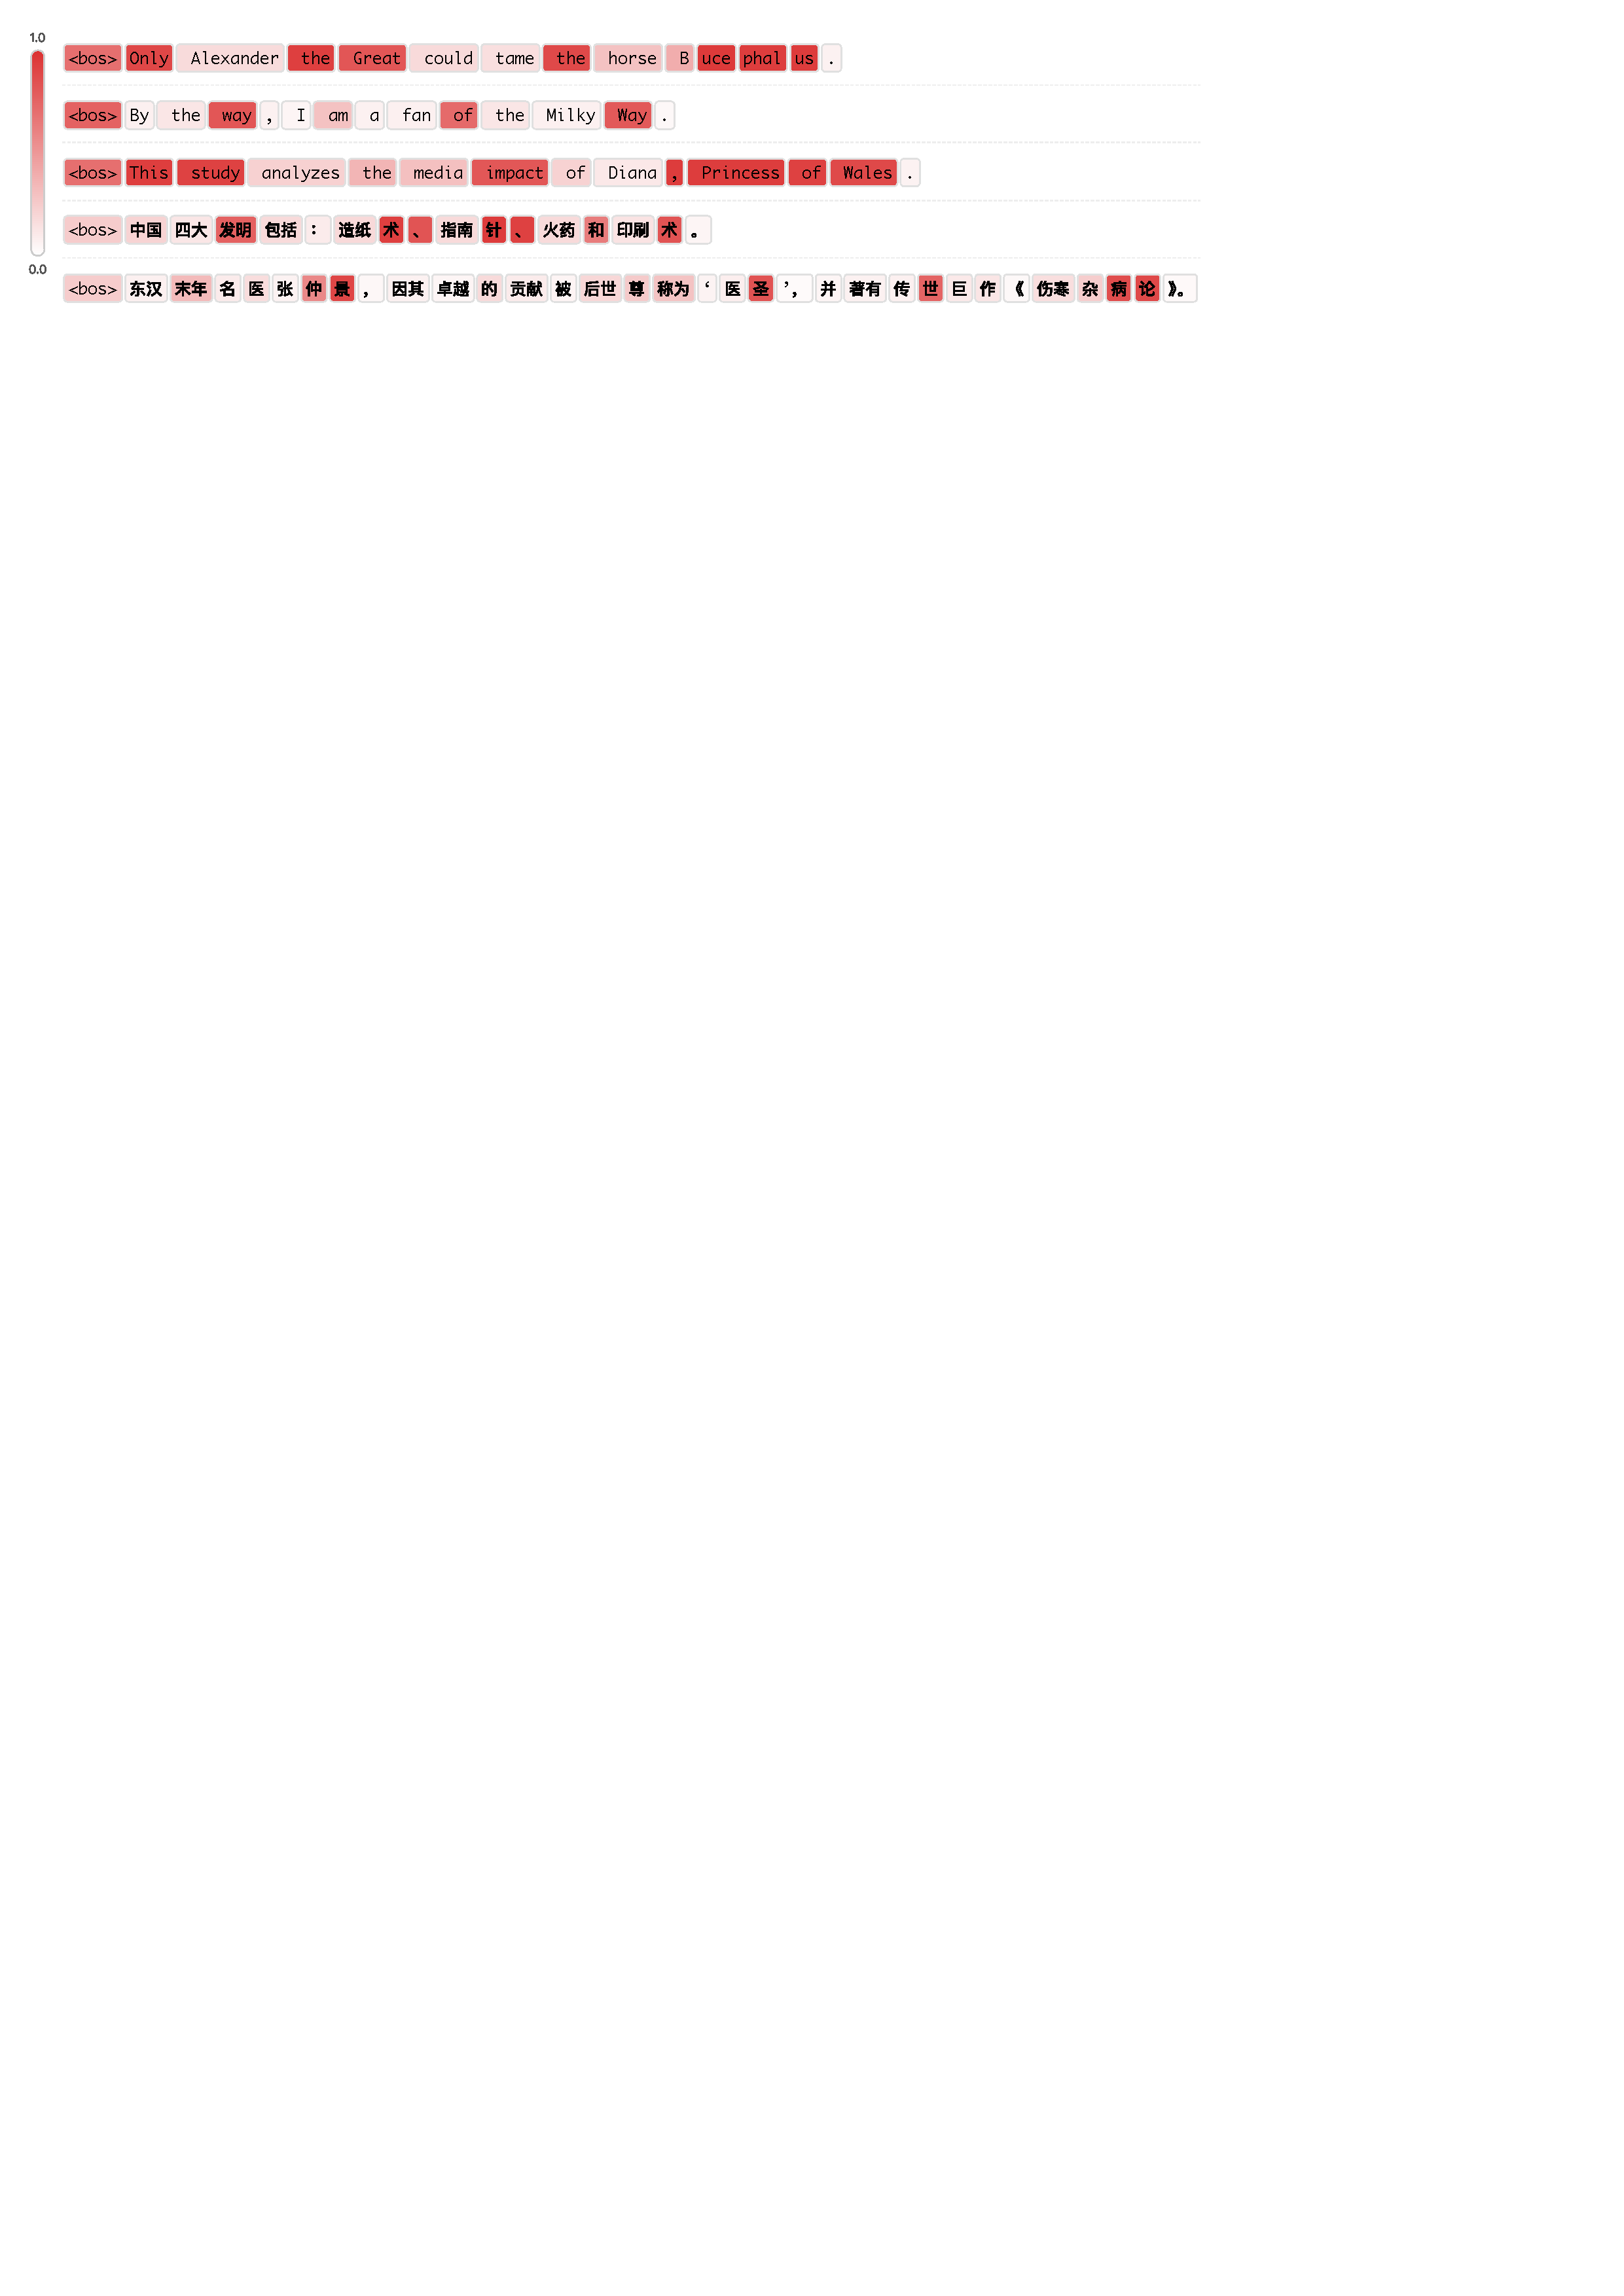
\includegraphics[width=\textwidth]{../papers/translations/engram/figures/visualization.pdf}
\caption{原文图7: Engram门控热图. 深红表示更大的$\alpha_t\in[0,1]$. 模块基于后缀$N$-gram,此处$N=3$,故token$x_t$上的强激活表示以它结尾的前序短语被识别为记忆中的静态模式. 图中五个完整样本在下文逐一保留,英语附中文翻译;图中子词切分、空格和$\langle\mathrm{bos}\rangle$是分词展示,不代表新增文本指令.}\label{engram-fig-7}
\end{figure}
完整样本如下;原文只给这些可视化序列, 没有另外公布逐字评测提示模板.
\begin{enumerate}
\item \texttt{<bos>} Only Alexander the Great could tame the horse Bucephalus.\par 只有亚历山大大帝能驯服名为Bucephalus的马.
\item \texttt{<bos>} By the way, I am a fan of the Milky Way.\par 顺便说一句, 我是银河的爱好者.
\item \texttt{<bos>} This study analyzes the media impact of Diana, Princess of Wales.\par 本研究分析威尔士王妃戴安娜的媒体影响.
\item \texttt{<bos>} 中国四大发明包括: 造纸术、指南针、火药和印刷术.
\item \texttt{<bos>} 东汉末年名医张仲景, 因其卓越的贡献被后世尊称为“医圣”, 并著有传世巨作《伤寒杂病论》.
\end{enumerate}

\originalsection{7 相关工作}\paperlabel{7}{engram-sec-7}
\phantomsection
\noindent\textbf{$N$-gram建模与embedding扩展.}\paperlabel{7}{engram-sec-7-1}
$N$-gram源于Shannon框架\cite{engram-shannon1948mathematical}, 依赖局部历史预测token, 传统方法用平滑\cite{engram-kneser1995improved,engram-DBLP:journals/tsp/Katz87}减轻数据稀疏. 虽然神经架构\cite{engram-bengio2003neural}取代其长程依赖建模, 查找效率仍保留在现代表征学习中, 如FastText\cite{engram-bojanowski2017enriching}.

近来该范式以embedding扩展形式复兴. Per-Layer Embeddings\cite{engram-gemma_3n_2025}、STEM\cite{engram-sadhukhan2026stem}、L3\cite{engram-tseng20263}、DeepEmbed\cite{engram-rwkv_deepembed_wiki_2025}用大表扩容量. 更接近我们的另一条工作线, 将组合$N$-gram直接融入表征空间. N-Grammer\cite{engram-roy2022n}用离散潜文本表示构建$N$-gram来增强Transformer; Feng等\cite{engram-feng2023memory}展示其语音识别效用. SuperBPE\cite{engram-liu2025superbpe}把高频多词表达合成“超词”token; SCONE\cite{engram-yu2025scaling}则用辅助编码模型. OverEncoding\cite{engram-huang2025over}与字节潜在Transformer(BLT)\cite{engram-pagnoni2025byte}分别用哈希token级和byte级$N$-gram embedding捕捉局部依赖. 这些工作共同显示, $N$-gram参数扩展可以只有很小计算开销. 我们在两方面有根本区别.

第一, 建模和评价协议不同. 既有方法常把$N$-gram当外部增强, 没在严格公平协议下验证效率. SCONE主要面向推断, 辅助模块增加训练FLOPs; 原文称OverEncoding即使在非等参数设置下, 也未在稀疏MoE骨干上带来有意义改善. 我们把条件记忆当一等原语, 用精心设计的Engram实现, 在稀疏分配框架中严格评价, 展示对等参数、等FLOPs的MoE基线优势.

第二, 系统上采用算法与系统共同设计. 既有方法把embedding严格放在输入层, 第0层, 使访问与计算串行\cite{engram-yu2025scaling,engram-huang2025over}. Engram放在更深层以重叠通信与计算. 再利用$N$-gram的Zipf分布, 可以充分利用存储层级. 作者认为整体设计能以可忽略推断开销扩展大量参数.

\phantomsection
\noindent\textbf{高基数类别embedding.}\paperlabel{7}{engram-sec-7-2}
推荐系统也有相关表征问题: 数百个类别特征的词表可能各有数百万到数十亿ID\cite{engram-coleman2023unified}. 既有方法通过多哈希和组合表示\cite{engram-tito2017hash,engram-shi2020compositional}、频率感知哈希和碰撞管理\cite{engram-zhang2020model,engram-tsang2022clustering,engram-zhang2024cafe}、频率/重要性自适应容量\cite{engram-ginart2021mixed,engram-joglekar2020neural,engram-liu2021learnable}, 以及量化、张量分解、共享内存布局的结构压缩\cite{engram-kang2020learning,engram-yin2021tt,engram-desai2021random}, 改善参数--准确率与访问权衡. 其他方法跨类别域共享表示\cite{engram-coleman2023unified}, 无显式表生成embedding\cite{engram-kang2021learning}, 或用学习到的语义标识代替任意物品ID\cite{engram-rajput2023recommender,engram-singh2024better}. Engram同样面对高度偏斜访问下的大离散键空间, 但键由有序文本$N$-gram构成, 通过上下文门控注入Transformer中间层.

\phantomsection
\noindent\textbf{混合专家.}\paperlabel{7}{engram-sec-7-3}
MoE通过每token条件激活少数专家, 分离容量与计算成本, 由Shazeer等提出\cite{engram-shazeer2017outrageously}. 后续GShard\cite{engram-lepikhin2020gshard}、BASE\cite{engram-pmlr-v139-lewis21a}、Switch Transformer\cite{engram-fedus2022switch}、GLaM\cite{engram-du2022glam}在保持固定推断成本时支持超线性参数扩展. 近期DeepSeek-MoE\cite{engram-dai2024deepseekmoe}借助细粒度专家分割与共享专家隔离, 显著优于同激活参数稠密模型. DeepSeek-V3\cite{engram-liu2024deepseek}与Kimi-k2\cite{engram-kimi-k2}采用这类架构, 总参数达数百十亿规模.

\phantomsection
\noindent\textbf{记忆网络.}\paperlabel{7}{engram-sec-7-4}
记忆增强研究旨在增加容量而不同比例增加计算, 大体分参数与非参数方法. 参数记忆如PKM\cite{engram-lample2019large}、PEER\cite{engram-he2024mixture}、Selfmem\cite{engram-cheng2023lift}、Memory+\cite{engram-berges2024memory}、UltraMem\cite{engram-huang2024ultra,engram-huang2025ultramemv2}, 将大规模稀疏键值存储直接加入模型层, 以很小FLOPs影响扩容量. 非参数记忆如REALM\cite{engram-guu2020retrieval}、RETRO\cite{engram-borgeaud2022improving,engram-wang2023shall}、CoG\cite{engram-lan2023copy,engram-caoretrieval}、PlugLM\cite{engram-cheng2023decouple}, 分离知识存储与处理, 把外部记忆视为可编辑、可扩展键值库, 适应变化信息而无需昂贵重训.

\phantomsection
\noindent\textbf{知识存储机制.}\paperlabel{7}{engram-sec-7-5}
容量扩展之外, 许多研究考察Transformer如何编码、取回事实知识. FFN被广泛假设为键值记忆\cite{engram-geva2021transformer}: 第一层探测模式作“键”, 第二层把特定信息作“值”投到残差流. 特定“知识神经元”的识别\cite{engram-dai2022knowledge}支持模块性. 因果跟踪\cite{engram-meng2022locating}把事实回忆信息流定位到特定FFN层, 提供进一步证据, 并启发ROME\cite{engram-meng2022locating}、MEMIT\cite{engram-meng2022mass}等无需重训直接更新事实关联的编辑算法. Othello-GPT等内部表示研究\cite{engram-li2024emergentworldrepresentationsexploring}还提示, 这些存储机制可能帮助形成结构化“世界模型”.

\originalsection{8 结论}\paperlabel{8}{engram-sec-8}
本工作提出条件记忆, 作为主流条件计算MoE的互补稀疏轴, 解决动态计算模拟知识检索的低效. Engram把经典$N$-gram embedding现代化, 实现对静态模式可扩展、常数时间$O(1)$查找.

建立稀疏分配问题后, 我们观察U形规律, 混合分配MoE专家与Engram容量严格优于纯MoE. 据此训练27B模型, 多领域性能更好; 记忆虽直观上有助知识检索, 一般推理、代码与数学收益也很大.

机制分析提示, Engram免去早期静态重建, 有效“加深”网络, 为全局上下文和复杂推理释放注意力. 结构改变在LongPPL与RULER中体现为长上下文改善. Engram还强调基础设施效率: 确定寻址分离存储与计算, 允许大表卸载到主机内存, 推断额外开销很小. 我们认为条件记忆将成为下一代稀疏模型不可缺少的建模原语.

\originalsection{附录 A: 完整架构与超参数}\paperlabel{A}{engram-app-A}
\begingroup\setlength{\tabcolsep}{3pt}
\begin{longtable}{p{.36\textwidth}cccc}
\caption{原文表5: 完整模型架构和训练超参数.}\label{engram-tab-5}\\
\toprule
 & \shortstack{Dense\\4B} & \shortstack{MoE\\27B} & \shortstack{Engram\\27B} & \shortstack{Engram\\40B} \\
\midrule
总参数 & 4.1B & 26.7B & 26.7B & 39.5B \\
激活参数 & \multicolumn{4}{c}{3.8B} \\
训练token数 & \multicolumn{4}{c}{262B} \\
\midrule
层数 & \multicolumn{4}{c}{30} \\
隐层维度 & \multicolumn{4}{c}{2560} \\
开头稠密层数 & - & 1 &1 &1 \\
路由专家数 & - & 72& 55 & 55 \\
激活专家数 & - & 6 & 6 & 6 \\
共享专家数 & - &2 & 2& 2\\
负载均衡方式 & - & \multicolumn{3}{c}{无辅助损失~\cite{engram-wang2024auxiliarylossfreeloadbalancingstrategy}} \\
\midrule
注意力模块 & \multicolumn{4}{c}{MLA~\cite{engram-deepseekai2024deepseekv2strongeconomicalefficient}} \\ 
RoPE $\theta$ & \multicolumn{4}{c}{10000} \\
mHC扩张率 & \multicolumn{4}{c}{4} \\
序列长度 & \multicolumn{4}{c}{4096} \\
词表大小 & \multicolumn{4}{c}{129280} \\
批量大小 & \multicolumn{4}{c}{1280} \\
训练步数 & \multicolumn{4}{c}{50000} \\
骨干优化器 & \multicolumn{4}{c}{Muon~\cite{engram-jordan2024muon}} \\
嵌入优化器 & \multicolumn{4}{c}{Adam~\cite{engram-kingma2014adam}} \\
基础学习率 & \multicolumn{4}{c}{4e-4} \\
学习率调度 & \multicolumn{4}{c}{分段衰减~\cite{engram-bi2024deepseek}} \\
权重衰减 & \multicolumn{4}{c}{0.1}  \\
\midrule
Engram维度 $d_{\text{mem}}$ & - & - & 1280 & 1280 \\
Engram槽数 & - & - & 2262400 & 7239680 \\
Engram头数 & - & - & 8 & 8 \\
Engram插入层 & - & - & [2,15] & [2,15] \\
Engram $N$-gram & - & - & [2,3] & [2,3] \\
Engram结合mHC & - & - & 是 & 是 \\
Engram分词器压缩  & - & - & 是 & 是 \\
Engram卷积零初始化  & - & - & 是 & 是 \\
Engram学习率倍数  & - & - & x5 & x5 \\
Engram权重衰减  & - & - & 0.0 & 0.0 \\
Engram优化器(仅嵌入)  & - & - & \multicolumn{2}{c}{Adam~\cite{engram-kingma2014adam}}  \\
\bottomrule
\end{longtable}
\endgroup


\clearpage
\originalsection{附录 B: 全部基准曲线}\paperlabel{B}{engram-app-B}
\begin{figure}[!ht]
\centering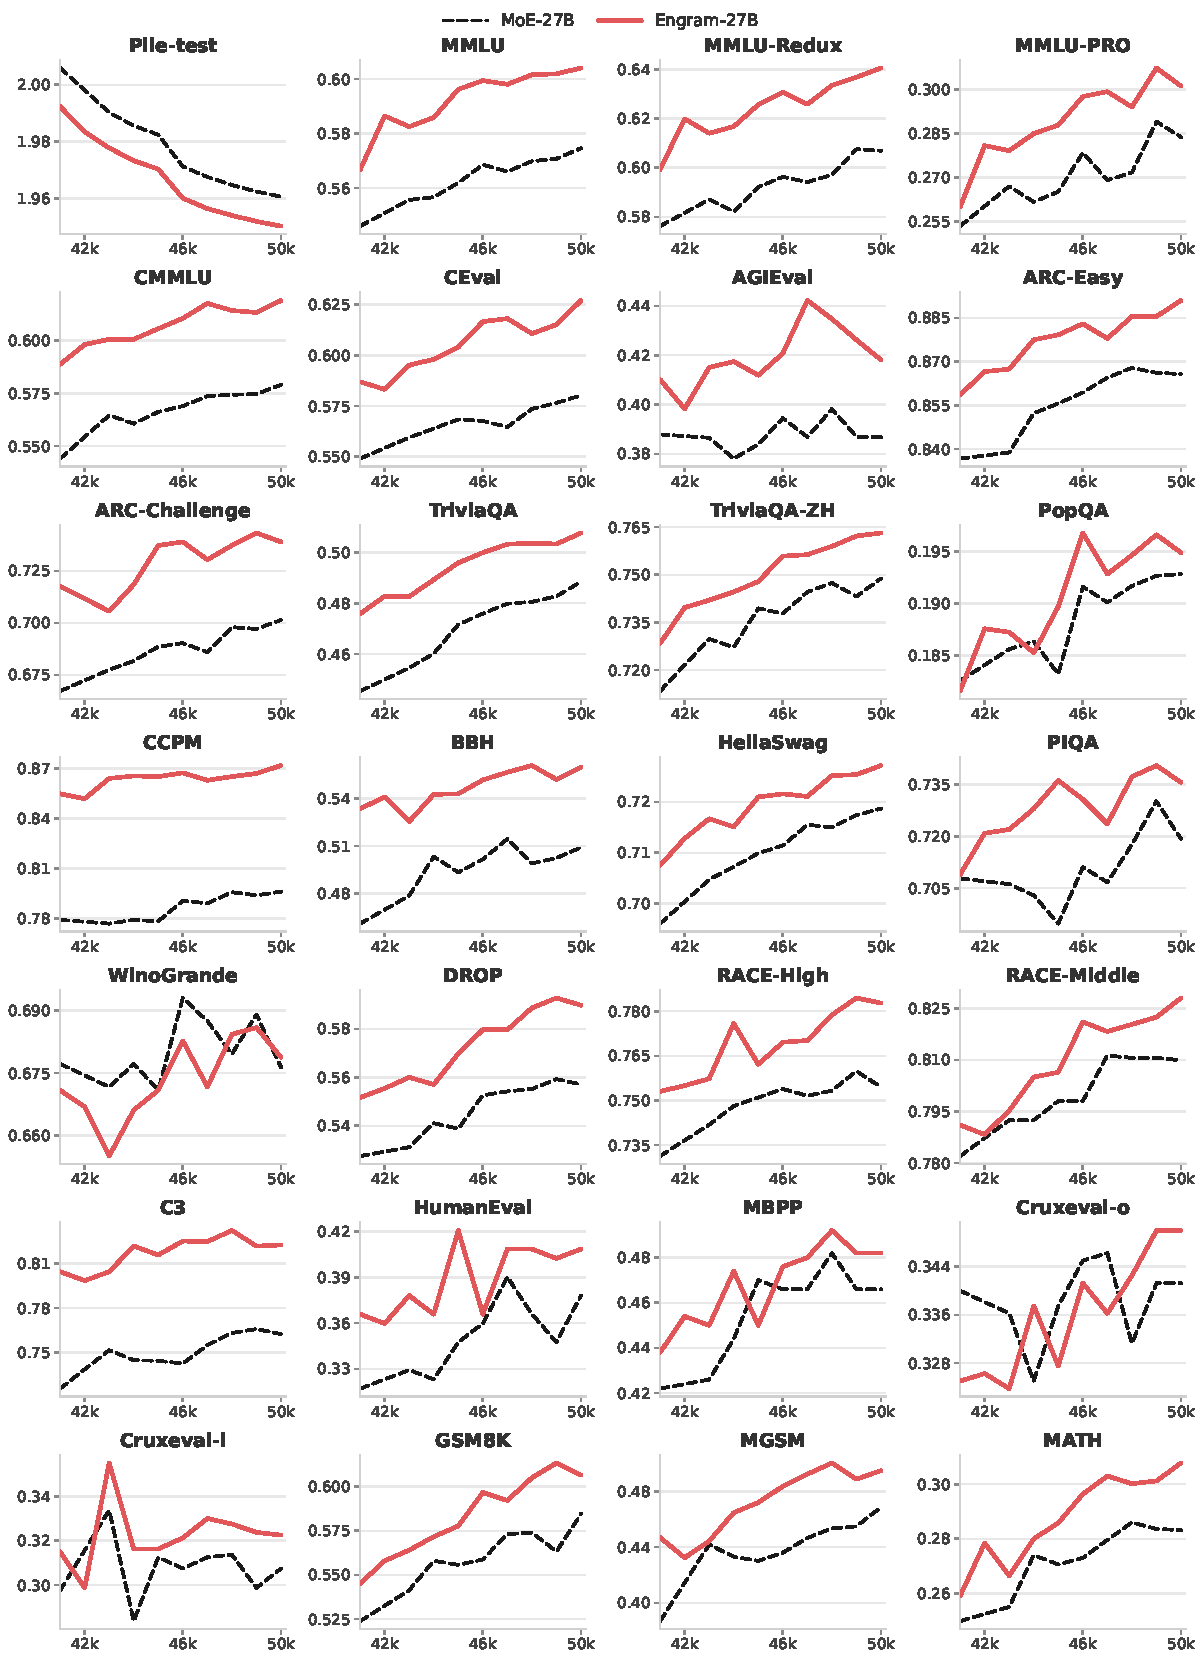
\includegraphics[width=.97\textwidth,height=.70\textheight,keepaspectratio]{../papers/translations/engram/figures/benchmark_curve.pdf}
\caption{原文图8: 预训练最后10k步的全部基准曲线. 原图包含Pile-test、MMLU、MMLU-Redux、MMLU-Pro、CMMLU、C-Eval、AGIEval、ARC-Easy、ARC-Challenge、TriviaQA、TriviaQA-ZH、PopQA、CCPM、BBH、HellaSwag、PIQA、WinoGrande、DROP、RACE-High、RACE-Middle、C3、HumanEval、MBPP、CruxEval-o/i、GSM8K、MGSM、MATH,图例为MoE-27B与Engram-27B. 横轴为训练步数,如42k、46k、50k;各纵轴沿用原图指标尺度. 图本身为完整矢量PDF,可放大检查细节.}\label{engram-fig-8}
\end{figure}

\clearpage
\originalsection{附录 C: 分词器压缩案例}\paperlabel{C}{engram-app-C}
\begin{table}[htbp]
\centering\begingroup\setlength{\tabcolsep}{3pt}
\caption{原文表6: 分词器压缩合并数最多的5个token. 128k分词器总体压缩率为23.43\%. 以下保留原文列出的所有原token与省略号;“\textvisiblespace”表示可见空格,反斜杠t/n/r为原表展示的制表/换行/回车形式.}\label{engram-tab-6}
\begin{tabular}{rrlp{.65\textwidth}}\toprule
排名 & 合并数 & 规范token & 原token\\\midrule
1 & 163 & \texttt{'\textvisiblespace'} & \texttt{'\textbackslash t'}, \texttt{'\textbackslash n'}, \texttt{'\textbackslash r'}, \texttt{'\textvisiblespace'}, \texttt{'\textvisiblespace\textvisiblespace'}, \texttt{'\textbackslash n\textbackslash n'}, \texttt{'\textvisiblespace\textvisiblespace\textvisiblespace'}, \texttt{'\textvisiblespace\textbackslash n'}, \ldots\\
2 & 54 & \texttt{'a'} & \texttt{'A'}, \texttt{'a'}, \texttt{'\textvisiblespace a'}, \texttt{'\textvisiblespace A'}, \texttt{'á'}, \texttt{'ä'}, \texttt{'ã'}, \texttt{'ą'}, \texttt{'\textvisiblespace à'}, \texttt{'\textvisiblespace å'}, \texttt{'â'}, \ldots\\
3 & 40 & \texttt{'o'} & \texttt{'O'}, \texttt{'o'}, \texttt{'\textvisiblespace o'}, \texttt{'\textvisiblespace O'}, \texttt{'ó'}, \texttt{'ö'}, \texttt{'ô'}, \texttt{'õ'}, \texttt{'ő'}, \texttt{'ò'}, \ldots\\
4 & 35 & \texttt{'e'} & \texttt{'E'}, \texttt{'e'}, \texttt{'\textvisiblespace e'}, \texttt{'\textvisiblespace E'}, \texttt{'é'}, \texttt{'è'}, \texttt{'\textvisiblespace é'}, \texttt{'ę'}, \texttt{'ě'}, \texttt{'ê'}, \ldots\\
5 & 30 & \texttt{'i'} & \texttt{'I'}, \texttt{'i'}, \texttt{'\textvisiblespace I'}, \texttt{'\textvisiblespace i'}, \texttt{'í'}, \texttt{'ì'}, \texttt{'î'}, \texttt{'ī'}, \texttt{'ï'}, \ldots\\\bottomrule
\end{tabular}\endgroup
\end{table}

\originalsection{译者核查注}\label{engram-translator-notes}
以下为译者补充, 不属于原论文. 本稿译出了指定版全部实质正文与附录, 原图、原表数字及原书目保留, 未把不一致默默改成一致.

第一, 摘要和引言的“MMLU $+3.4$”与主表的$57.4\to60.4$, 即$+3.0$, 不一致; 主表MMLU-Redux恰为$60.6\to64.0$, 即$+3.4$. 结果节用$+3.0$. 本稿保留各处原报告. 附录B部分曲线也不能直接作为主表逐点复算依据;例如C3曲线的可见刻度约0.75--0.81,与主表MoE/Engram的60.1/63.6不在相同数值区间,原文未解释这一差异.

第二, 长上下文段落“所有指标更好”“全面最高”“单调改善”等概括并非逐项成立. 等损失46k的单针S为97.6,低于MoE的100.0; CWE为4.3,低于4.5. QA在41k为44.0,46k为37.5,50k为40.5,并不单调; FWE为99.6、98.6、99.3,也非单调. 全表数值及作者粗体/下划线保留,其标记也不总严格对应最大值. 相同预训练损失是一项控制,不保证所有潜在基础能力和历史都相同.

第三, $\mathcal O(1)$ 指固定阶数和哈希头数下的查找工作不随表槽数增长,不是全部硬件访问延迟或通信开销的无条件常数保证. 100B卸载吞吐实测仅限H800、512序列、长度Uniform$(100,1024)$、4B/8B稠密骨干及该原型实现. 原文对多级缓存和更大规模的讨论包含设计主张与外推,不是已报告每种硬件/每种负载都小于3\%开销.

第四, “无限记忆”是放宽参数预算的有限扫描,最大槽数$10^7$,并非真正无限. 作者将扩展曲线同时描述为“对数线性”与“严格幂律”;对数横轴上的原损失近似直线,与原损失本身满足幂律是不同函数形式,还需定义拟合量、不可约损失和误差. 原文措辞保留,不把有限扫描提升为渐近定理.

第五, LogitLens与CKA提供表征/读出相关性证据,不单独证明唯一因果机制、计算图等价或真实层数增加. 较低的中间到最终分布KL衡量一致性,并不保证最终预测正确. 有限批次的无偏HSIC估计及其比值也不能仅据人口版本结论保证所有估计CKA都严格落在$[0,1]$. 软对齐还需要分母非零和top-$k$平票处理,原文未详述这些边界.

第六, 门控可视化明确挑选了语义匹配相关最强的分支,不是全部8门值的随机样本. 事后抑制记忆引入训练--推断分布变化,保留原性能比例不是同等训练预算下重训消融结果;两点均已按原文保留. 门值点积自身也不提供语义冲突必然被阻断的数学保证.

第七, Engram表为可训练参数,训练中用Adam更新;“静态”主要区别于由隐状态动态计算地址,不能据此把它当成无需学习或可任意编辑而无需验证的外部事实库. 卷积零初始化在式 \eqref{engram-eq-5} 中给$\mathbf Y=\tilde{\mathbf V}$,故仅凭卷积为零不能推出整个Engram残差输出为零;原文恒等映射表述须区分卷积子模块与整模块.

第八, 官方arXiv作者条目写Yixu Wei,指定PDF/source写Yixuan Wei. 正文作者表按PDF/source保留,元数据记录两种原写法. Source系统图文件名为\texttt{Engram\_system.pdf},引用路径却写小写;译稿仅规范文件名大小写. 部分原BibTeX条目缺年份或期刊,本稿保留原书目内容并在核查记录标出,没有猜测补全. 原文没有独立限制节或正式定理/证明/算法环境,不虚构作者未给的证明或逐字提示模板.

% 指定版实际引用的135项完整原书目;保持原文检索信息.
\begin{thebibliography}{135}
\providecommand{\natexlab}[1]{#1}
\providecommand{\url}[1]{\texttt{#1}}
\expandafter\ifx\csname urlstyle\endcsname\relax
  \providecommand{\doi}[1]{doi: #1}\else
  \providecommand{\doi}{doi: \begingroup \urlstyle{rm}\Url}\fi

\bibitem{engram-austin2021program}
J.~Austin, A.~Odena, M.~Nye, M.~Bosma, H.~Michalewski, D.~Dohan, E.~Jiang,
  C.~Cai, M.~Terry, Q.~Le, et~al.
\newblock Program synthesis with large language models.
\newblock \emph{arXiv preprint arXiv:2108.07732}, 2021.

\bibitem{engram-bahdanau2014neural}
D.~Bahdanau, K.~Cho, and Y.~Bengio.
\newblock Neural machine translation by jointly learning to align and
  translate.
\newblock In Y.~Bengio and Y.~LeCun, editors, \emph{3rd International
  Conference on Learning Representations, {ICLR} 2015, San Diego, CA, USA, May
  7-9, 2015, Conference Track Proceedings}, 2015.
\newblock URL \url{http://arxiv.org/abs/1409.0473}.

\bibitem{engram-belrose2023eliciting}
N.~Belrose, Z.~Furman, L.~Smith, D.~Halawi, I.~Ostrovsky, L.~McKinney,
  S.~Biderman, and J.~Steinhardt.
\newblock Eliciting latent predictions from transformers with the tuned lens.
\newblock \emph{arXiv preprint arXiv:2303.08112}, 2023.

\bibitem{engram-bengio2003neural}
Y.~Bengio, R.~Ducharme, P.~Vincent, and C.~Janvin.
\newblock A neural probabilistic language model.
\newblock \emph{J. Mach. Learn. Res.}, 3:\penalty0 1137--1155, 2003.
\newblock URL \url{https://jmlr.org/papers/v3/bengio03a.html}.

\bibitem{engram-bengio2013estimatingpropagatinggradientsstochastic}
Y.~Bengio, N.~Léonard, and A.~Courville.
\newblock Estimating or propagating gradients through stochastic neurons for
  conditional computation, 2013.
\newblock URL \url{https://arxiv.org/abs/1308.3432}.

\bibitem{engram-berges2024memory}
V.~Berges, B.~Oguz, D.~Haziza, W.~Yih, L.~Zettlemoyer, and G.~Ghosh.
\newblock Memory layers at scale.
\newblock In \emph{Forty-second International Conference on Machine Learning,
  {ICML} 2025, Vancouver, BC, Canada, July 13-19, 2025}. OpenReview.net, 2025.
\newblock URL \url{https://openreview.net/forum?id=ATqGm1WyDj}.

\bibitem{engram-bi2024deepseek}
X.~Bi, D.~Chen, G.~Chen, S.~Chen, D.~Dai, C.~Deng, H.~Ding, K.~Dong, Q.~Du,
  Z.~Fu, et~al.
\newblock Deepseek llm: Scaling open-source language models with longtermism.
\newblock \emph{arXiv preprint arXiv:2401.02954}, 2024.

\bibitem{engram-bisk2020piqa}
Y.~Bisk, R.~Zellers, J.~Gao, Y.~Choi, et~al.
\newblock Piqa: Reasoning about physical commonsense in natural language.
\newblock In \emph{Proceedings of the AAAI conference on artificial
  intelligence}, volume~34, pages 7432--7439, 2020.

\bibitem{engram-bojanowski2017enriching}
P.~Bojanowski, E.~Grave, A.~Joulin, and T.~Mikolov.
\newblock Enriching word vectors with subword information.
\newblock \emph{Transactions of the association for computational linguistics},
  5:\penalty0 135--146, 2017.

\bibitem{engram-borgeaud2022improving}
S.~Borgeaud, A.~Mensch, J.~Hoffmann, T.~Cai, E.~Rutherford, K.~Millican, G.~B.
  Van Den~Driessche, J.-B. Lespiau, B.~Damoc, A.~Clark, et~al.
\newblock Improving language models by retrieving from trillions of tokens.
\newblock In \emph{International conference on machine learning}, pages
  2206--2240. PMLR, 2022.

\bibitem{engram-brants-etal-2007-large}
T.~Brants, A.~C. Popat, P.~Xu, F.~J. Och, and J.~Dean.
\newblock Large language models in machine translation.
\newblock In J.~Eisner, editor, \emph{Proceedings of the 2007 Joint Conference
  on Empirical Methods in Natural Language Processing and Computational Natural
  Language Learning ({EMNLP}-{C}o{NLL})}, pages 858--867, Prague, Czech
  Republic, June 2007. Association for Computational Linguistics.
\newblock URL \url{https://aclanthology.org/D07-1090/}.

\bibitem{engram-caoretrieval}
B.~Cao, D.~Cai, L.~Cui, X.~Cheng, W.~Bi, Y.~Zou, and S.~Shi.
\newblock Retrieval is accurate generation.
\newblock In \emph{The Twelfth International Conference on Learning
  Representations}.

\bibitem{engram-Chao1950HumanBA}
Y.~R. Chao and G.~K. Zipf.
\newblock Human behavior and the principle of least effort: An introduction to
  human ecology.
\newblock \emph{Language}, 26:\penalty0 394, 1950.
\newblock URL \url{https://api.semanticscholar.org/CorpusID:10182796}.

\bibitem{engram-chen2021evaluatinglargelanguagemodels}
M.~Chen, J.~Tworek, H.~Jun, Q.~Yuan, H.~P. de~Oliveira~Pinto, J.~Kaplan,
  H.~Edwards, Y.~Burda, N.~Joseph, G.~Brockman, A.~Ray, R.~Puri, G.~Krueger,
  M.~Petrov, H.~Khlaaf, G.~Sastry, P.~Mishkin, B.~Chan, S.~Gray, N.~Ryder,
  M.~Pavlov, A.~Power, L.~Kaiser, M.~Bavarian, C.~Winter, P.~Tillet, F.~P.
  Such, D.~Cummings, M.~Plappert, F.~Chantzis, E.~Barnes, A.~Herbert-Voss,
  W.~H. Guss, A.~Nichol, A.~Paino, N.~Tezak, J.~Tang, I.~Babuschkin, S.~Balaji,
  S.~Jain, W.~Saunders, C.~Hesse, A.~N. Carr, J.~Leike, J.~Achiam, V.~Misra,
  E.~Morikawa, A.~Radford, M.~Knight, M.~Brundage, M.~Murati, K.~Mayer,
  P.~Welinder, B.~McGrew, D.~Amodei, S.~McCandlish, I.~Sutskever, and
  W.~Zaremba.
\newblock Evaluating large language models trained on code, 2021.
\newblock URL \url{https://arxiv.org/abs/2107.03374}.

\bibitem{engram-cheng2023decouple}
X.~Cheng, Y.~Lin, X.~Chen, D.~Zhao, and R.~Yan.
\newblock Decouple knowledge from paramters for plug-and-play language
  modeling.
\newblock In A.~Rogers, J.~Boyd-Graber, and N.~Okazaki, editors, \emph{Findings
  of the Association for Computational Linguistics: ACL 2023}, pages
  14288--14308, Toronto, Canada, July 2023{\natexlab{a}}. Association for
  Computational Linguistics.
\newblock \doi{10.18653/v1/2023.findings-acl.901}.
\newblock URL \url{https://aclanthology.org/2023.findings-acl.901/}.

\bibitem{engram-cheng2023lift}
X.~Cheng, D.~Luo, X.~Chen, L.~Liu, D.~Zhao, and R.~Yan.
\newblock Lift yourself up: Retrieval-augmented text generation with
  self-memory.
\newblock \emph{Advances in Neural Information Processing Systems},
  36:\penalty0 43780--43799, 2023{\natexlab{b}}.

\bibitem{engram-clark2018think}
P.~Clark, I.~Cowhey, O.~Etzioni, T.~Khot, A.~Sabharwal, C.~Schoenick, and
  O.~Tafjord.
\newblock Think you have solved question answering? try arc, the ai2 reasoning
  challenge.
\newblock \emph{arXiv preprint arXiv:1803.05457}, 2018.

\bibitem{engram-cobbe2021training}
K.~Cobbe, V.~Kosaraju, M.~Bavarian, M.~Chen, H.~Jun, L.~Kaiser, M.~Plappert,
  J.~Tworek, J.~Hilton, R.~Nakano, et~al.
\newblock Training verifiers to solve math word problems.
\newblock \emph{arXiv preprint arXiv:2110.14168}, 2021.

\bibitem{engram-coleman2023unified}
B.~Coleman, W.-C. Kang, M.~Fahrbach, R.~Wang, L.~Hong, E.~Chi, and D.~Cheng.
\newblock Unified embedding: Battle-tested feature representations for
  web-scale ml systems.
\newblock \emph{Advances in Neural Information Processing Systems},
  36:\penalty0 56234--56255, 2023.

\bibitem{engram-comanici2025gemini}
G.~Comanici, E.~Bieber, M.~Schaekermann, I.~Pasupat, N.~Sachdeva, I.~Dhillon,
  M.~Blistein, O.~Ram, D.~Zhang, E.~Rosen, et~al.
\newblock Gemini 2.5: Pushing the frontier with advanced reasoning,
  multimodality, long context, and next generation agentic capabilities.
\newblock \emph{arXiv preprint arXiv:2507.06261}, 2025.

\bibitem{engram-constant2017survey}
M.~Constant, G.~Eryi{\u{g}}it, J.~Monti, L.~Van Der~Plas, C.~Ramisch,
  M.~Rosner, and A.~Todirascu.
\newblock Survey: multiword expression processing: a survey.
\newblock \emph{Computational Linguistics}, 43\penalty0 (4):\penalty0 837--892,
  2017.

\bibitem{engram-csordas2025language}
R.~Csord{\'a}s, C.~D. Manning, and C.~Potts.
\newblock Do language models use their depth efficiently?
\newblock \emph{arXiv preprint arXiv:2505.13898}, 2025.

\bibitem{engram-dai2022knowledge}
D.~Dai, L.~Dong, Y.~Hao, Z.~Sui, B.~Chang, and F.~Wei.
\newblock Knowledge neurons in pretrained transformers.
\newblock In \emph{Proceedings of the 60th Annual Meeting of the Association
  for Computational Linguistics (Volume 1: Long Papers)}, pages 8493--8502,
  2022.

\bibitem{engram-dai2024deepseekmoe}
D.~Dai, C.~Deng, C.~Zhao, R.~Xu, H.~Gao, D.~Chen, J.~Li, W.~Zeng, X.~Yu, Y.~Wu,
  et~al.
\newblock Deepseekmoe: Towards ultimate expert specialization in
  mixture-of-experts language models.
\newblock \emph{arXiv preprint arXiv:2401.06066}, 2024.

\bibitem{engram-davari2022reliability}
M.~Davari, S.~Horoi, A.~Natik, G.~Lajoie, G.~Wolf, and E.~Belilovsky.
\newblock Reliability of {CKA} as a similarity measure in deep learning.
\newblock In \emph{The Eleventh International Conference on Learning
  Representations, {ICLR} 2023, Kigali, Rwanda, May 1-5, 2023}. OpenReview.net,
  2023.
\newblock URL \url{https://openreview.net/forum?id=8HRvyxc606}.

\bibitem{engram-deepseekai2024deepseekv2strongeconomicalefficient}
DeepSeek-AI.
\newblock Deepseek-v2: A strong, economical, and efficient mixture-of-experts
  language model, 2024.
\newblock URL \url{https://arxiv.org/abs/2405.04434}.

\bibitem{engram-pmlr-v202-dehghani23a}
M.~Dehghani, J.~Djolonga, B.~Mustafa, P.~Padlewski, J.~Heek, J.~Gilmer, A.~P.
  Steiner, M.~Caron, R.~Geirhos, I.~Alabdulmohsin, R.~Jenatton, L.~Beyer,
  M.~Tschannen, A.~Arnab, X.~Wang, C.~Riquelme~Ruiz, M.~Minderer,
  J.~Puigcerver, U.~Evci, M.~Kumar, S.~V. Steenkiste, G.~F. Elsayed,
  A.~Mahendran, F.~Yu, A.~Oliver, F.~Huot, J.~Bastings, M.~Collier, A.~A.
  Gritsenko, V.~Birodkar, C.~N. Vasconcelos, Y.~Tay, T.~Mensink, A.~Kolesnikov,
  F.~Pavetic, D.~Tran, T.~Kipf, M.~Lucic, X.~Zhai, D.~Keysers, J.~J. Harmsen,
  and N.~Houlsby.
\newblock Scaling vision transformers to 22 billion parameters.
\newblock In A.~Krause, E.~Brunskill, K.~Cho, B.~Engelhardt, S.~Sabato, and
  J.~Scarlett, editors, \emph{Proceedings of the 40th International Conference
  on Machine Learning}, volume 202 of \emph{Proceedings of Machine Learning
  Research}, pages 7480--7512. PMLR, 23--29 Jul 2023.
\newblock URL \url{https://proceedings.mlr.press/v202/dehghani23a.html}.

\bibitem{engram-desai2021random}
A.~Desai, L.~Chou, and A.~Shrivastava.
\newblock Random offset block embedding array (robe) for criteotb benchmark
  mlperf dlrm model : 1000$\times$ compression and 3.1$\times$ faster
  inference, 2022.
\newblock URL \url{https://arxiv.org/abs/2108.02191}.

\bibitem{engram-ding2021few}
N.~Ding, G.~Xu, Y.~Chen, X.~Wang, X.~Han, P.~Xie, H.~Zheng, and Z.~Liu.
\newblock Few-nerd: A few-shot named entity recognition dataset.
\newblock In \emph{Proceedings of the 59th Annual Meeting of the Association
  for Computational Linguistics and the 11th International Joint Conference on
  Natural Language Processing (Volume 1: Long Papers)}, pages 3198--3213, 2021.

\bibitem{engram-du2022glam}
N.~Du, Y.~Huang, A.~M. Dai, S.~Tong, D.~Lepikhin, Y.~Xu, M.~Krikun, Y.~Zhou,
  A.~W. Yu, O.~Firat, et~al.
\newblock Glam: Efficient scaling of language models with mixture-of-experts.
\newblock In \emph{International conference on machine learning}, pages
  5547--5569. PMLR, 2022.

\bibitem{engram-dua2019drop}
D.~Dua, Y.~Wang, P.~Dasigi, G.~Stanovsky, S.~Singh, and M.~Gardner.
\newblock {DROP:} {A} reading comprehension benchmark requiring discrete
  reasoning over paragraphs.
\newblock In J.~Burstein, C.~Doran, and T.~Solorio, editors, \emph{Proceedings
  of the 2019 Conference of the North American Chapter of the Association for
  Computational Linguistics: Human Language Technologies, {NAACL-HLT} 2019,
  Minneapolis, MN, USA, June 2-7, 2019, Volume 1 (Long and Short Papers)},
  pages 2368--2378. Association for Computational Linguistics, 2019.
\newblock \doi{10.18653/V1/N19-1246}.
\newblock URL \url{https://doi.org/10.18653/v1/n19-1246}.

\bibitem{engram-elfwing2018sigmoid}
S.~Elfwing, E.~Uchibe, and K.~Doya.
\newblock Sigmoid-weighted linear units for neural network function
  approximation in reinforcement learning.
\newblock \emph{Neural networks}, 107:\penalty0 3--11, 2018.

\bibitem{engram-erman2000idiom}
B.~Erman.
\newblock The idiom principle and the open choice principle.
\newblock \emph{Text-Interdisciplinary Journal for the Study of Discourse},
  2000.

\bibitem{engram-fangwrong}
L.~Fang, Y.~Wang, Z.~Liu, C.~Zhang, S.~Jegelka, J.~Gao, B.~Ding, and Y.~Wang.
\newblock What is wrong with perplexity for long-context language modeling?
\newblock In \emph{The Thirteenth International Conference on Learning
  Representations}.

\bibitem{engram-fedus2022switch}
W.~Fedus, B.~Zoph, and N.~Shazeer.
\newblock Switch transformers: Scaling to trillion parameter models with simple
  and efficient sparsity.
\newblock \emph{Journal of Machine Learning Research}, 23\penalty0
  (120):\penalty0 1--39, 2022.

\bibitem{engram-feng2023memory}
Y.~Feng, M.~Tu, R.~Xia, C.~Huang, and Y.~Wang.
\newblock Memory augmented lookup dictionary based language modeling for
  automatic speech recognition.
\newblock In \emph{Proc. Interspeech 2023}, pages 481--485, 2023.

\bibitem{engram-gao2020pile}
L.~Gao, S.~Biderman, S.~Black, L.~Golding, T.~Hoppe, C.~Foster, J.~Phang,
  H.~He, A.~Thite, N.~Nabeshima, et~al.
\newblock The pile: An 800gb dataset of diverse text for language modeling.
\newblock \emph{arXiv preprint arXiv:2101.00027}, 2020.

\bibitem{engram-gao2025train}
T.~Gao, A.~Wettig, H.~Yen, and D.~Chen.
\newblock How to train long-context language models (effectively).
\newblock In \emph{Proceedings of the 63rd Annual Meeting of the Association
  for Computational Linguistics (Volume 1: Long Papers)}, pages 7376--7399,
  2025.

\bibitem{engram-gema2025we}
A.~P. Gema, J.~O.~J. Leang, G.~Hong, A.~Devoto, A.~C.~M. Mancino, R.~Saxena,
  X.~He, Y.~Zhao, X.~Du, M.~R.~G. Madani, et~al.
\newblock Are we done with mmlu?
\newblock In \emph{Proceedings of the 2025 Conference of the Nations of the
  Americas Chapter of the Association for Computational Linguistics: Human
  Language Technologies (Volume 1: Long Papers)}, pages 5069--5096, 2025.

\bibitem{engram-geva2021transformer}
M.~Geva, R.~Schuster, J.~Berant, and O.~Levy.
\newblock Transformer feed-forward layers are key-value memories.
\newblock In \emph{Proceedings of the 2021 Conference on Empirical Methods in
  Natural Language Processing}, pages 5484--5495, 2021.

\bibitem{engram-ghandeharioun2024patchscopes}
A.~Ghandeharioun, A.~Caciularu, A.~Pearce, L.~Dixon, and M.~Geva.
\newblock Patchscopes: A unifying framework for inspecting hidden
  representations of language models.
\newblock In \emph{International Conference on Machine Learning}, pages
  15466--15490. PMLR, 2024.

\bibitem{engram-ginart2021mixed}
A.~A. Ginart, M.~Naumov, D.~Mudigere, J.~Yang, and J.~Zou.
\newblock Mixed dimension embeddings with application to memory-efficient
  recommendation systems.
\newblock In \emph{2021 IEEE International symposium on information theory
  (ISIT)}, pages 2786--2791. IEEE, 2021.

\bibitem{engram-gretton2005measuring}
A.~Gretton, O.~Bousquet, A.~Smola, and B.~Sch{\"o}lkopf.
\newblock Measuring statistical dependence with hilbert-schmidt norms.
\newblock In \emph{International conference on algorithmic learning theory},
  pages 63--77. Springer, 2005.

\bibitem{engram-gu2021efficiently}
A.~Gu, K.~Goel, and C.~R{\'{e}}.
\newblock Efficiently modeling long sequences with structured state spaces.
\newblock In \emph{The Tenth International Conference on Learning
  Representations, {ICLR} 2022, Virtual Event, April 25-29, 2022}.
  OpenReview.net, 2022.
\newblock URL \url{https://openreview.net/forum?id=uYLFoz1vlAC}.

\bibitem{engram-gu2024cruxeval}
A.~Gu, B.~Rozi{\`{e}}re, H.~J. Leather, A.~Solar{-}Lezama, G.~Synnaeve, and
  S.~Wang.
\newblock Cruxeval: {A} benchmark for code reasoning, understanding and
  execution.
\newblock In \emph{Forty-first International Conference on Machine Learning,
  {ICML} 2024, Vienna, Austria, July 21-27, 2024}. OpenReview.net, 2024.
\newblock URL \url{https://openreview.net/forum?id=Ffpg52swvg}.

\bibitem{engram-guo2025deepseek}
D.~Guo, D.~Yang, H.~Zhang, J.~Song, R.~Zhang, R.~Xu, Q.~Zhu, S.~Ma, P.~Wang,
  X.~Bi, et~al.
\newblock Deepseek-r1: Incentivizing reasoning capability in llms via
  reinforcement learning.
\newblock \emph{arXiv preprint arXiv:2501.12948}, 2025.

\bibitem{engram-guu2020retrieval}
K.~Guu, K.~Lee, Z.~Tung, P.~Pasupat, and M.~Chang.
\newblock Retrieval augmented language model pre-training.
\newblock In \emph{International conference on machine learning}, pages
  3929--3938. PMLR, 2020.

\bibitem{engram-haber-poesio-2024-polysemy}
J.~Haber and M.~Poesio.
\newblock {P}olysemy{---}{E}vidence from linguistics, behavioral science, and
  contextualized language models.
\newblock \emph{Computational Linguistics}, 50\penalty0 (1):\penalty0 351--417,
  Mar. 2024.
\newblock \doi{10.1162/coli_a_00500}.
\newblock URL \url{https://aclanthology.org/2024.cl-1.10/}.

\bibitem{engram-he2016deep}
K.~He, X.~Zhang, S.~Ren, and J.~Sun.
\newblock Deep residual learning for image recognition.
\newblock In \emph{Proceedings of the IEEE conference on computer vision and
  pattern recognition}, pages 770--778, 2016.

\bibitem{engram-he2024mixture}
X.~O. He.
\newblock Mixture of a million experts.
\newblock \emph{arXiv preprint arXiv:2407.04153}, 2024.

\bibitem{engram-hendrycks2020measuring}
D.~Hendrycks, C.~Burns, S.~Basart, A.~Zou, M.~Mazeika, D.~Song, and
  J.~Steinhardt.
\newblock Measuring massive multitask language understanding.
\newblock In \emph{9th International Conference on Learning Representations,
  {ICLR} 2021, Virtual Event, Austria, May 3-7, 2021}. OpenReview.net,
  2021{\natexlab{a}}.
\newblock URL \url{https://openreview.net/forum?id=d7KBjmI3GmQ}.

\bibitem{engram-hendrycks2021measuring}
D.~Hendrycks, C.~Burns, S.~Kadavath, A.~Arora, S.~Basart, E.~Tang, D.~Song, and
  J.~Steinhardt.
\newblock Measuring mathematical problem solving with the {MATH} dataset.
\newblock In J.~Vanschoren and S.~Yeung, editors, \emph{Proceedings of the
  Neural Information Processing Systems Track on Datasets and Benchmarks 1,
  NeurIPS Datasets and Benchmarks 2021, December 2021, virtual},
  2021{\natexlab{b}}.
\newblock URL
  \url{https://datasets-benchmarks-proceedings.neurips.cc/paper/2021/hash/be83ab3ecd0db773eb2dc1b0a17836a1-Abstract-round2.html}.

\bibitem{engram-hsiehruler}
C.-P. Hsieh, S.~Sun, S.~Kriman, S.~Acharya, D.~Rekesh, F.~Jia, and B.~Ginsburg.
\newblock Ruler: What’s the real context size of your long-context language
  models?
\newblock In \emph{First Conference on Language Modeling}.

\bibitem{engram-huang2025over}
H.~Huang, D.~Zhu, B.~Wu, Y.~Zeng, Y.~Wang, Q.~Min, and X.~Zhou.
\newblock Over-tokenized transformer: Vocabulary is generally worth scaling.
\newblock In \emph{Forty-second International Conference on Machine Learning,
  {ICML} 2025, Vancouver, BC, Canada, July 13-19, 2025}. OpenReview.net,
  2025{\natexlab{a}}.
\newblock URL \url{https://openreview.net/forum?id=gbeZKej40m}.

\bibitem{engram-huang2023c}
Y.~Huang, Y.~Bai, Z.~Zhu, J.~Zhang, J.~Zhang, T.~Su, J.~Liu, C.~Lv, Y.~Zhang,
  Y.~Fu, et~al.
\newblock C-eval: A multi-level multi-discipline chinese evaluation suite for
  foundation models.
\newblock \emph{Advances in Neural Information Processing Systems},
  36:\penalty0 62991--63010, 2023.

\bibitem{engram-huang2025ultramemv2}
Z.~Huang, Y.~Bao, Q.~Min, S.~Chen, R.~Guo, H.~Huang, D.~Zhu, Y.~Zeng, B.~Wu,
  X.~Zhou, et~al.
\newblock Ultramemv2: Memory networks scaling to 120b parameters with superior
  long-context learning.
\newblock \emph{arXiv preprint arXiv:2508.18756}, 2025{\natexlab{b}}.

\bibitem{engram-huang2024ultra}
Z.~Huang, Q.~Min, H.~Huang, Y.~Zeng, D.~Zhu, R.~Guo, and X.~Zhou.
\newblock Ultra-sparse memory network.
\newblock In \emph{The Thirteenth International Conference on Learning
  Representations, {ICLR} 2025, Singapore, April 24-28, 2025}. OpenReview.net,
  2025{\natexlab{c}}.
\newblock URL \url{https://openreview.net/forum?id=zjeHLSiNv1}.

\bibitem{engram-DBLP:conf/coling/JinYHZWH0MMDYDZ25}
M.~Jin, Q.~Yu, J.~Huang, Q.~Zeng, Z.~Wang, W.~Hua, H.~Zhao, K.~Mei, Y.~Meng,
  K.~Ding, F.~Yang, M.~Du, and Y.~Zhang.
\newblock Exploring concept depth: How large language models acquire knowledge
  and concept at different layers?
\newblock In O.~Rambow, L.~Wanner, M.~Apidianaki, H.~Al{-}Khalifa, B.~D.
  Eugenio, and S.~Schockaert, editors, \emph{Proceedings of the 31st
  International Conference on Computational Linguistics, {COLING} 2025, Abu
  Dhabi, UAE, January 19-24, 2025}, pages 558--573. Association for
  Computational Linguistics, 2025.
\newblock URL \url{https://aclanthology.org/2025.coling-main.37/}.

\bibitem{engram-joglekar2020neural}
M.~R. Joglekar, C.~Li, M.~Chen, T.~Xu, X.~Wang, J.~K. Adams, P.~Khaitan,
  J.~Liu, and Q.~V. Le.
\newblock Neural input search for large scale recommendation models.
\newblock In \emph{Proceedings of the 26th ACM SIGKDD International Conference
  on Knowledge Discovery \& Data Mining}, pages 2387--2397, 2020.

\bibitem{engram-jordan2024muon}
K.~Jordan, Y.~Jin, V.~Boza, J.~You, F.~Cesista, L.~Newhouse, and J.~Bernstein.
\newblock Muon: An optimizer for hidden layers in neural networks, 2024.
\newblock URL \url{https://kellerjordan.github.io/posts/muon/}.

\bibitem{engram-joshi2017triviaqa}
M.~Joshi, E.~Choi, D.~S. Weld, and L.~Zettlemoyer.
\newblock Triviaqa: {A} large scale distantly supervised challenge dataset for
  reading comprehension.
\newblock In R.~Barzilay and M.~Kan, editors, \emph{Proceedings of the 55th
  Annual Meeting of the Association for Computational Linguistics, {ACL} 2017,
  Vancouver, Canada, July 30 - August 4, Volume 1: Long Papers}, pages
  1601--1611. Association for Computational Linguistics, 2017.
\newblock \doi{10.18653/V1/P17-1147}.
\newblock URL \url{https://doi.org/10.18653/v1/P17-1147}.

\bibitem{engram-kang2020learning}
W.-C. Kang, D.~Z. Cheng, T.~Chen, X.~Yi, D.~Lin, L.~Hong, and E.~H. Chi.
\newblock Learning multi-granular quantized embeddings for large-vocab
  categorical features in recommender systems.
\newblock In \emph{Companion Proceedings of the Web Conference 2020}, pages
  562--566, 2020.

\bibitem{engram-kang2021learning}
W.-C. Kang, D.~Z. Cheng, T.~Yao, X.~Yi, T.~Chen, L.~Hong, and E.~H. Chi.
\newblock Learning to embed categorical features without embedding tables for
  recommendation.
\newblock In \emph{Proceedings of the 27th ACM SIGKDD Conference on Knowledge
  Discovery \& Data Mining}, pages 840--850, 2021.

\bibitem{engram-DBLP:journals/tsp/Katz87}
S.~M. Katz.
\newblock Estimation of probabilities from sparse data for the language model
  component of a speech recognizer.
\newblock \emph{{IEEE} Trans. Acoust. Speech Signal Process.}, 35\penalty0
  (3):\penalty0 400--401, 1987.
\newblock \doi{10.1109/TASSP.1987.1165125}.
\newblock URL \url{https://doi.org/10.1109/TASSP.1987.1165125}.

\bibitem{engram-kimi-k2}
Kimi.
\newblock Kimi {K2:} open agentic intelligence.
\newblock \emph{CoRR}, abs/2507.20534, 2025.
\newblock \doi{10.48550/ARXIV.2507.20534}.
\newblock URL \url{https://doi.org/10.48550/arXiv.2507.20534}.

\bibitem{engram-kingma2014adam}
D.~P. Kingma.
\newblock Adam: A method for stochastic optimization.
\newblock \emph{arXiv preprint arXiv:1412.6980}, 2014.

\bibitem{engram-kneser1995improved}
R.~Kneser and H.~Ney.
\newblock Improved backing-off for m-gram language modeling.
\newblock In \emph{1995 international conference on acoustics, speech, and
  signal processing}, volume~1, pages 181--184. IEEE, 1995.

\bibitem{engram-kornblith2019similarity}
S.~Kornblith, M.~Norouzi, H.~Lee, and G.~Hinton.
\newblock Similarity of neural network representations revisited.
\newblock In \emph{International conference on machine learning}, pages
  3519--3529. PMlR, 2019.

\bibitem{engram-kriegeskorte2008representational}
N.~Kriegeskorte, M.~Mur, and P.~A. Bandettini.
\newblock Representational similarity analysis-connecting the branches of
  systems neuroscience.
\newblock \emph{Frontiers in systems neuroscience}, 2:\penalty0 249, 2008.

\bibitem{engram-kudo2018sentencepiecesimplelanguageindependent}
T.~Kudo and J.~Richardson.
\newblock Sentencepiece: {A} simple and language independent subword tokenizer
  and detokenizer for neural text processing.
\newblock In E.~Blanco and W.~Lu, editors, \emph{Proceedings of the 2018
  Conference on Empirical Methods in Natural Language Processing, {EMNLP} 2018:
  System Demonstrations, Brussels, Belgium, October 31 - November 4, 2018},
  pages 66--71. Association for Computational Linguistics, 2018.
\newblock \doi{10.18653/V1/D18-2012}.
\newblock URL \url{https://doi.org/10.18653/v1/d18-2012}.

\bibitem{engram-kullback1951information}
S.~Kullback and R.~A. Leibler.
\newblock On information and sufficiency.
\newblock \emph{The annals of mathematical statistics}, 22\penalty0
  (1):\penalty0 79--86, 1951.

\bibitem{engram-kwon2023efficient}
W.~Kwon, Z.~Li, S.~Zhuang, Y.~Sheng, L.~Zheng, C.~H. Yu, J.~Gonzalez, H.~Zhang,
  and I.~Stoica.
\newblock Efficient memory management for large language model serving with
  pagedattention.
\newblock In \emph{Proceedings of the 29th symposium on operating systems
  principles}, pages 611--626, 2023.

\bibitem{engram-lai2017race}
G.~Lai, Q.~Xie, H.~Liu, Y.~Yang, and E.~H. Hovy.
\newblock {RACE:} large-scale reading comprehension dataset from examinations.
\newblock In M.~Palmer, R.~Hwa, and S.~Riedel, editors, \emph{Proceedings of
  the 2017 Conference on Empirical Methods in Natural Language Processing,
  {EMNLP} 2017, Copenhagen, Denmark, September 9-11, 2017}, pages 785--794.
  Association for Computational Linguistics, 2017.
\newblock \doi{10.18653/V1/D17-1082}.
\newblock URL \url{https://doi.org/10.18653/v1/d17-1082}.

\bibitem{engram-lample2019large}
G.~Lample, A.~Sablayrolles, M.~Ranzato, L.~Denoyer, and H.~J{\'e}gou.
\newblock Large memory layers with product keys.
\newblock \emph{Advances in Neural Information Processing Systems}, 32, 2019.

\bibitem{engram-lan2023copy}
T.~Lan, D.~Cai, Y.~Wang, H.~Huang, and X.-L. Mao.
\newblock Copy is all you need.
\newblock \emph{arXiv preprint arXiv:2307.06962}, 2023.

\bibitem{engram-larsson2016fractalnet}
G.~Larsson, M.~Maire, and G.~Shakhnarovich.
\newblock Fractalnet: Ultra-deep neural networks without residuals.
\newblock In \emph{5th International Conference on Learning Representations,
  {ICLR} 2017, Toulon, France, April 24-26, 2017, Conference Track
  Proceedings}. OpenReview.net, 2017.
\newblock URL \url{https://openreview.net/forum?id=S1VaB4cex}.

\bibitem{engram-lennie2003cost}
P.~Lennie.
\newblock The cost of cortical computation.
\newblock \emph{Current biology}, 13\penalty0 (6):\penalty0 493--497, 2003.

\bibitem{engram-lepikhin2020gshard}
D.~Lepikhin, H.~Lee, Y.~Xu, D.~Chen, O.~Firat, Y.~Huang, M.~Krikun, N.~Shazeer,
  and Z.~Chen.
\newblock Gshard: Scaling giant models with conditional computation and
  automatic sharding.
\newblock \emph{arXiv preprint arXiv:2006.16668}, 2020.

\bibitem{engram-pmlr-v139-lewis21a}
M.~Lewis, S.~Bhosale, T.~Dettmers, N.~Goyal, and L.~Zettlemoyer.
\newblock Base layers: Simplifying training of large, sparse models.
\newblock In M.~Meila and T.~Zhang, editors, \emph{Proceedings of the 38th
  International Conference on Machine Learning}, volume 139 of
  \emph{Proceedings of Machine Learning Research}, pages 6265--6274. PMLR,
  18--24 Jul 2021.
\newblock URL \url{https://proceedings.mlr.press/v139/lewis21a.html}.

\bibitem{engram-li2024cmmlu}
H.~Li, Y.~Zhang, F.~Koto, Y.~Yang, H.~Zhao, Y.~Gong, N.~Duan, and T.~Baldwin.
\newblock Cmmlu: Measuring massive multitask language understanding in chinese.
\newblock In \emph{Findings of the Association for Computational Linguistics:
  ACL 2024}, pages 11260--11285, 2024.

\bibitem{engram-li2024emergentworldrepresentationsexploring}
K.~Li, A.~K. Hopkins, D.~Bau, F.~B. Vi{\'{e}}gas, H.~Pfister, and
  M.~Wattenberg.
\newblock Emergent world representations: Exploring a sequence model trained on
  a synthetic task.
\newblock In \emph{The Eleventh International Conference on Learning
  Representations, {ICLR} 2023, Kigali, Rwanda, May 1-5, 2023}. OpenReview.net,
  2023{\natexlab{a}}.
\newblock URL \url{https://openreview.net/forum?id=DeG07\_TcZvT}.

\bibitem{engram-li2025echoesbertmodernlanguage}
M.~Li and N.~Subramani.
\newblock Echoes of bert: Do modern language models rediscover the classical
  nlp pipeline?, 2025.
\newblock URL \url{https://arxiv.org/abs/2506.02132}.

\bibitem{engram-li2023starcodersourceyou}
R.~Li, L.~B. Allal, Y.~Zi, N.~Muennighoff, D.~Kocetkov, C.~Mou, M.~Marone,
  C.~Akiki, J.~Li, J.~Chim, Q.~Liu, E.~Zheltonozhskii, T.~Y. Zhuo, T.~Wang,
  O.~Dehaene, M.~Davaadorj, J.~Lamy{-}Poirier, J.~Monteiro, O.~Shliazhko,
  N.~Gontier, N.~Meade, A.~Zebaze, M.~Yee, L.~K. Umapathi, J.~Zhu, B.~Lipkin,
  M.~Oblokulov, Z.~Wang, R.~M. V, J.~T. Stillerman, S.~S. Patel, D.~Abulkhanov,
  M.~Zocca, M.~Dey, Z.~Zhang, N.~Fahmy, U.~Bhattacharyya, W.~Yu, S.~Singh,
  S.~Luccioni, P.~Villegas, M.~Kunakov, F.~Zhdanov, M.~Romero, T.~Lee,
  N.~Timor, J.~Ding, C.~Schlesinger, H.~Schoelkopf, J.~Ebert, T.~Dao,
  M.~Mishra, A.~Gu, J.~Robinson, C.~J. Anderson, B.~Dolan{-}Gavitt,
  D.~Contractor, S.~Reddy, D.~Fried, D.~Bahdanau, Y.~Jernite, C.~M. Ferrandis,
  S.~Hughes, T.~Wolf, A.~Guha, L.~von Werra, and H.~de~Vries.
\newblock Starcoder: may the source be with you!
\newblock \emph{Trans. Mach. Learn. Res.}, 2023, 2023{\natexlab{b}}.
\newblock URL \url{https://openreview.net/forum?id=KoFOg41haE}.

\bibitem{engram-li2021ccpm}
W.~Li, F.~Qi, M.~Sun, X.~Yi, and J.~Zhang.
\newblock Ccpm: A chinese classical poetry matching dataset.
\newblock \emph{arXiv preprint arXiv:2106.01979}, 2021.

\bibitem{engram-liu2024deepseek}
A.~Liu, B.~Feng, B.~Xue, B.~Wang, B.~Wu, C.~Lu, C.~Zhao, C.~Deng, C.~Zhang,
  C.~Ruan, et~al.
\newblock Deepseek-v3 technical report.
\newblock \emph{arXiv preprint arXiv:2412.19437}, 2024{\natexlab{a}}.

\bibitem{engram-liu2025superbpe}
A.~Liu, J.~Hayase, V.~Hofmann, S.~Oh, N.~A. Smith, and Y.~Choi.
\newblock Super{BPE}: Space travel for language models.
\newblock In \emph{Second Conference on Language Modeling}, 2025{\natexlab{a}}.
\newblock URL \url{https://openreview.net/forum?id=lcDRvffeNP}.

\bibitem{engram-liu2024infini}
J.~Liu, S.~Min, L.~Zettlemoyer, Y.~Choi, and H.~Hajishirzi.
\newblock Infini-gram: Scaling unbounded n-gram language models to a trillion
  tokens.
\newblock In \emph{First Conference on Language Modeling}, 2024{\natexlab{b}}.
\newblock URL \url{https://openreview.net/forum?id=u2vAyMeLMm}.

\bibitem{engram-liu2025muon}
J.~Liu, J.~Su, X.~Yao, Z.~Jiang, G.~Lai, Y.~Du, Y.~Qin, W.~Xu, E.~Lu, J.~Yan,
  et~al.
\newblock Muon is scalable for llm training.
\newblock \emph{arXiv preprint arXiv:2502.16982}, 2025{\natexlab{b}}.

\bibitem{engram-liu2021learnable}
S.~Liu, C.~Gao, Y.~Chen, D.~Jin, and Y.~Li.
\newblock Learnable embedding sizes for recommender systems.
\newblock \emph{arXiv preprint arXiv:2101.07577}, 2021.

\bibitem{engram-mallen2023not}
A.~Mallen, A.~Asai, V.~Zhong, R.~Das, D.~Khashabi, and H.~Hajishirzi.
\newblock When not to trust language models: Investigating effectiveness of
  parametric and non-parametric memories.
\newblock In \emph{Proceedings of the 61st Annual Meeting of the Association
  for Computational Linguistics (Volume 1: Long Papers)}, pages 9802--9822,
  2023.

\bibitem{engram-meng2022locating}
K.~Meng, D.~Bau, A.~Andonian, and Y.~Belinkov.
\newblock Locating and editing factual associations in gpt.
\newblock \emph{Advances in neural information processing systems},
  35:\penalty0 17359--17372, 2022.

\bibitem{engram-meng2022mass}
K.~Meng, A.~S. Sharma, A.~J. Andonian, Y.~Belinkov, and D.~Bau.
\newblock Mass-editing memory in a transformer.
\newblock In \emph{The Eleventh International Conference on Learning
  Representations, {ICLR} 2023, Kigali, Rwanda, May 1-5, 2023}. OpenReview.net,
  2023.
\newblock URL \url{https://openreview.net/forum?id=MkbcAHIYgyS}.

\bibitem{engram-nguyen2024understanding}
T.~Nguyen.
\newblock Understanding transformers via n-gram statistics.
\newblock \emph{Advances in neural information processing systems},
  37:\penalty0 98049--98082, 2024.

\bibitem{engram-nostalgebraist2020logitlens}
nostalgebraist.
\newblock interpreting gpt: the logit lens.
\newblock \emph{LessWrong}, 2020.
\newblock URL
  \url{https://www.lesswrong.com/posts/AcKRB8wDpdaN6v6ru/interpreting-gpt-the-logit-lens}.

\bibitem{engram-olshausen1997sparse}
B.~A. Olshausen and D.~J. Field.
\newblock Sparse coding with an overcomplete basis set: A strategy employed by
  v1?
\newblock \emph{Vision research}, 37\penalty0 (23):\penalty0 3311--3325, 1997.

\bibitem{engram-pagnoni2025byte}
A.~Pagnoni, R.~Pasunuru, P.~Rodriguez, J.~Nguyen, B.~Muller, M.~Li, C.~Zhou,
  L.~Yu, J.~E. Weston, L.~Zettlemoyer, et~al.
\newblock Byte latent transformer: Patches scale better than tokens.
\newblock In \emph{Proceedings of the 63rd Annual Meeting of the Association
  for Computational Linguistics (Volume 1: Long Papers)}, pages 9238--9258,
  2025.

\bibitem{engram-peng2023rwkv}
B.~Peng, E.~Alcaide, Q.~Anthony, A.~Albalak, S.~Arcadinho, S.~Biderman, H.~Cao,
  X.~Cheng, M.~Chung, L.~Derczynski, X.~Du, M.~Grella, K.~K. GV, X.~He, H.~Hou,
  P.~Kazienko, J.~Kocon, J.~Kong, B.~Koptyra, H.~Lau, J.~Lin, K.~S.~I. Mantri,
  F.~Mom, A.~Saito, G.~Song, X.~Tang, J.~S. Wind, S.~Wozniak, Z.~Zhang,
  Q.~Zhou, J.~Zhu, and R.~Zhu.
\newblock {RWKV:} reinventing rnns for the transformer era.
\newblock In H.~Bouamor, J.~Pino, and K.~Bali, editors, \emph{Findings of the
  Association for Computational Linguistics: {EMNLP} 2023, Singapore, December
  6-10, 2023}, pages 14048--14077. Association for Computational Linguistics,
  2023.
\newblock \doi{10.18653/V1/2023.FINDINGS-EMNLP.936}.
\newblock URL \url{https://doi.org/10.18653/v1/2023.findings-emnlp.936}.

\bibitem{engram-peng2023yarn}
B.~Peng, J.~Quesnelle, H.~Fan, and E.~Shippole.
\newblock Yarn: Efficient context window extension of large language models.
\newblock In \emph{The Twelfth International Conference on Learning
  Representations, {ICLR} 2024, Vienna, Austria, May 7-11, 2024}.
  OpenReview.net, 2024.
\newblock URL \url{https://openreview.net/forum?id=wHBfxhZu1u}.

\bibitem{engram-piantadosi2014zipf}
S.~T. Piantadosi.
\newblock Zipf’s word frequency law in natural language: A critical review
  and future directions.
\newblock \emph{Psychonomic bulletin \& review}, 21\penalty0 (5):\penalty0
  1112--1130, 2014.

\bibitem{engram-press2021train}
O.~Press, N.~A. Smith, and M.~Lewis.
\newblock Train short, test long: Attention with linear biases enables input
  length extrapolation.
\newblock In \emph{The Tenth International Conference on Learning
  Representations, {ICLR} 2022, Virtual Event, April 25-29, 2022}.
  OpenReview.net, 2022.
\newblock URL \url{https://openreview.net/forum?id=R8sQPpGCv0}.

\bibitem{engram-rajput2023recommender}
S.~Rajput, N.~Mehta, A.~Singh, R.~Hulikal~Keshavan, T.~Vu, L.~Heldt, L.~Hong,
  Y.~Tay, V.~Tran, J.~Samost, et~al.
\newblock Recommender systems with generative retrieval.
\newblock \emph{Advances in Neural Information Processing Systems},
  36:\penalty0 10299--10315, 2023.

\bibitem{engram-roy2022n}
A.~Roy, R.~Anil, G.~Lai, B.~Lee, J.~Zhao, S.~Zhang, S.~Wang, Y.~Zhang, S.~Wu,
  R.~Swavely, et~al.
\newblock N-grammer: Augmenting transformers with latent n-grams.
\newblock \emph{arXiv preprint arXiv:2207.06366}, 2022.

\bibitem{engram-rwkv_deepembed_wiki_2025}
{RWKV Team}.
\newblock Rwkv architecture history.
\newblock \url{https://wiki.rwkv.com/basic/architecture.html}, 2025.
\newblock Section ``RWKV-V8's DeepEmbed'', accessed 2025-12-09.

\bibitem{engram-sadhukhan2026stem}
R.~Sadhukhan, S.~Cao, H.~Dong, C.~Zhao, A.~Purpura-Pontoniere, Y.~Tian, Z.~Liu,
  and B.~Chen.
\newblock Stem: Scaling transformers with embedding modules.
\newblock \emph{arXiv preprint arXiv:2601.10639}, 2026.

\bibitem{engram-sakaguchi2021winogrande}
K.~Sakaguchi, R.~L. Bras, C.~Bhagavatula, and Y.~Choi.
\newblock Winogrande: An adversarial winograd schema challenge at scale.
\newblock \emph{Communications of the ACM}, 64\penalty0 (9):\penalty0 99--106,
  2021.

\bibitem{engram-shannon1948mathematical}
C.~E. Shannon.
\newblock A mathematical theory of communication.
\newblock \emph{The Bell system technical journal}, 27\penalty0 (3):\penalty0
  379--423, 1948.

\bibitem{engram-shazeer2017outrageously}
N.~Shazeer, A.~Mirhoseini, K.~Maziarz, A.~Davis, Q.~Le, G.~Hinton, and J.~Dean.
\newblock Outrageously large neural networks: The sparsely-gated
  mixture-of-experts layer.
\newblock \emph{arXiv preprint arXiv:1701.06538}, 2017.

\bibitem{engram-shi2022language}
F.~Shi, M.~Suzgun, M.~Freitag, X.~Wang, S.~Srivats, S.~Vosoughi, H.~W. Chung,
  Y.~Tay, S.~Ruder, D.~Zhou, D.~Das, and J.~Wei.
\newblock Language models are multilingual chain-of-thought reasoners.
\newblock In \emph{The Eleventh International Conference on Learning
  Representations, {ICLR} 2023, Kigali, Rwanda, May 1-5, 2023}. OpenReview.net,
  2023.
\newblock URL \url{https://openreview.net/forum?id=fR3wGCk-IXp}.

\bibitem{engram-shi2020compositional}
H.-J.~M. Shi, D.~Mudigere, M.~Naumov, and J.~Yang.
\newblock Compositional embeddings using complementary partitions for
  memory-efficient recommendation systems.
\newblock In \emph{Proceedings of the 26th ACM SIGKDD International Conference
  on Knowledge Discovery \& Data Mining}, pages 165--175, 2020.

\bibitem{engram-singh2024better}
A.~Singh, T.~Vu, N.~Mehta, R.~Keshavan, M.~Sathiamoorthy, Y.~Zheng, L.~Hong,
  L.~Heldt, L.~Wei, D.~Tandon, et~al.
\newblock Better generalization with semantic ids: A case study in ranking for
  recommendations.
\newblock In \emph{Proceedings of the 18th ACM Conference on Recommender
  Systems}, pages 1039--1044, 2024.

\bibitem{engram-su2023roformerenhancedtransformerrotary}
J.~Su, M.~H.~M. Ahmed, Y.~Lu, S.~Pan, W.~Bo, and Y.~Liu.
\newblock Roformer: Enhanced transformer with rotary position embedding.
\newblock \emph{Neurocomputing}, 568:\penalty0 127063, 2024.
\newblock \doi{10.1016/J.NEUCOM.2023.127063}.
\newblock URL \url{https://doi.org/10.1016/j.neucom.2023.127063}.

\bibitem{engram-sun2020investigating}
K.~Sun, D.~Yu, D.~Yu, and C.~Cardie.
\newblock Investigating prior knowledge for challenging chinese machine reading
  comprehension.
\newblock \emph{Transactions of the Association for Computational Linguistics},
  8:\penalty0 141--155, 2020.

\bibitem{engram-suzgun2023challenging}
M.~Suzgun, N.~Scales, N.~Sch{\"a}rli, S.~Gehrmann, Y.~Tay, H.~W. Chung,
  A.~Chowdhery, Q.~Le, E.~Chi, D.~Zhou, et~al.
\newblock Challenging big-bench tasks and whether chain-of-thought can solve
  them.
\newblock In \emph{Findings of the Association for Computational Linguistics:
  ACL 2023}, pages 13003--13051, 2023.

\bibitem{engram-szegedy2015going}
C.~Szegedy, W.~Liu, Y.~Jia, P.~Sermanet, S.~Reed, D.~Anguelov, D.~Erhan,
  V.~Vanhoucke, and A.~Rabinovich.
\newblock Going deeper with convolutions.
\newblock In \emph{Proceedings of the IEEE conference on computer vision and
  pattern recognition}, pages 1--9, 2015.

\bibitem{engram-gemma_3n_2025}
G.~Team.
\newblock Gemma 3n.
\newblock 2025.
\newblock URL \url{https://ai.google.dev/gemma/docs/gemma-3n}.

\bibitem{engram-tenney2019bert}
I.~Tenney, D.~Das, and E.~Pavlick.
\newblock Bert rediscovers the classical nlp pipeline.
\newblock In \emph{Proceedings of the 57th Annual Meeting of the Association
  for Computational Linguistics}. Association for Computational Linguistics,
  2019.

\bibitem{engram-tito2017hash}
D.~Tito~Svenstrup, J.~Hansen, and O.~Winther.
\newblock Hash embeddings for efficient word representations.
\newblock \emph{Advances in neural information processing systems}, 30, 2017.

\bibitem{engram-tsang2022clustering}
H.~L.-H. Tsang and T.~D. Ahle.
\newblock Clustering the sketch: A novel approach to embedding table
  compression.
\newblock \emph{arXiv preprint arXiv:2210.05974}, 2022.

\bibitem{engram-tseng20263}
A.~Tseng and C.~D. Sa.
\newblock L$^3$: Large lookup layers, 2026.
\newblock URL \url{https://arxiv.org/abs/2601.21461}.

\bibitem{engram-vaswani2017attention}
A.~Vaswani, N.~Shazeer, N.~Parmar, J.~Uszkoreit, L.~Jones, A.~N. Gomez,
  {\L}.~Kaiser, and I.~Polosukhin.
\newblock Attention is all you need.
\newblock \emph{Advances in neural information processing systems}, 30, 2017.

\bibitem{engram-wang2023shall}
B.~Wang, W.~Ping, P.~Xu, L.~McAfee, Z.~Liu, M.~Shoeybi, Y.~Dong, O.~Kuchaiev,
  B.~Li, C.~Xiao, et~al.
\newblock Shall we pretrain autoregressive language models with retrieval? a
  comprehensive study.
\newblock In \emph{Proceedings of the 2023 conference on empirical methods in
  natural language processing}, pages 7763--7786, 2023.

\bibitem{engram-wang2024auxiliarylossfreeloadbalancingstrategy}
L.~Wang, H.~Gao, C.~Zhao, X.~Sun, and D.~Dai.
\newblock Auxiliary-loss-free load balancing strategy for mixture-of-experts,
  2024{\natexlab{a}}.
\newblock URL \url{https://arxiv.org/abs/2408.15664}.

\bibitem{engram-wang2024mmlu}
Y.~Wang, X.~Ma, G.~Zhang, Y.~Ni, A.~Chandra, S.~Guo, W.~Ren, A.~Arulraj, X.~He,
  Z.~Jiang, et~al.
\newblock Mmlu-pro: A more robust and challenging multi-task language
  understanding benchmark.
\newblock \emph{Advances in Neural Information Processing Systems},
  37:\penalty0 95266--95290, 2024{\natexlab{b}}.

\bibitem{engram-UAX15-NFKC}
K.~Whistler.
\newblock Unicode standard annex \#15: Unicode normalization forms.
\newblock Unicode Standard Annex~15, The Unicode Consortium, July 2025.
\newblock URL \url{https://www.unicode.org/reports/tr15/tr15-57.html}.
\newblock Version Unicode 17.0.0, Revision 57. Accessed 2026-01-04.

\bibitem{engram-xiao2023efficient}
G.~Xiao, Y.~Tian, B.~Chen, S.~Han, and M.~Lewis.
\newblock Efficient streaming language models with attention sinks.
\newblock In \emph{The Twelfth International Conference on Learning
  Representations, {ICLR} 2024, Vienna, Austria, May 7-11, 2024}.
  OpenReview.net, 2024.
\newblock URL \url{https://openreview.net/forum?id=NG7sS51zVF}.

\bibitem{engram-xie2025mhcmanifoldconstrainedhyperconnections}
Z.~Xie, Y.~Wei, H.~Cao, C.~Zhao, C.~Deng, J.~Li, D.~Dai, H.~Gao, J.~Chang,
  L.~Zhao, S.~Zhou, Z.~Xu, Z.~Zhang, W.~Zeng, S.~Hu, Y.~Wang, J.~Yuan, L.~Wang,
  and W.~Liang.
\newblock mhc: Manifold-constrained hyper-connections, 2025.
\newblock URL \url{https://arxiv.org/abs/2512.24880}.

\bibitem{engram-yang2025path}
S.~Yang, Y.~Shen, K.~Wen, S.~Tan, M.~Mishra, L.~Ren, R.~Panda, and Y.~Kim.
\newblock Path attention: Position encoding via accumulating householder
  transformations.
\newblock \emph{arXiv preprint arXiv:2505.16381}, 2025.

\bibitem{engram-yin2021tt}
C.~Yin, B.~Acun, C.-J. Wu, and X.~Liu.
\newblock Tt-rec: Tensor train compression for deep learning recommendation
  models.
\newblock \emph{Proceedings of Machine Learning and Systems}, 3:\penalty0
  448--462, 2021.

\bibitem{engram-yu2025scaling}
D.~Yu, E.~Cohen, B.~Ghazi, Y.~Huang, P.~Kamath, R.~Kumar, D.~Liu, and C.~Zhang.
\newblock Scaling embedding layers in language models.
\newblock \emph{arXiv preprint arXiv:2502.01637}, 2025.

\bibitem{engram-zellers2019hellaswag}
R.~Zellers, A.~Holtzman, Y.~Bisk, A.~Farhadi, and Y.~Choi.
\newblock Hellaswag: Can a machine really finish your sentence?
\newblock In A.~Korhonen, D.~R. Traum, and L.~M{\`{a}}rquez, editors,
  \emph{Proceedings of the 57th Conference of the Association for Computational
  Linguistics, {ACL} 2019, Florence, Italy, July 28- August 2, 2019, Volume 1:
  Long Papers}, pages 4791--4800. Association for Computational Linguistics,
  2019.
\newblock \doi{10.18653/V1/P19-1472}.
\newblock URL \url{https://doi.org/10.18653/v1/p19-1472}.

\bibitem{engram-zhang2019root}
B.~Zhang and R.~Sennrich.
\newblock Root mean square layer normalization.
\newblock \emph{Advances in neural information processing systems}, 32, 2019.

\bibitem{engram-zhang2020model}
C.~Zhang, Y.~Liu, Y.~Xie, S.~I. Ktena, A.~Tejani, A.~Gupta, P.~K. Myana,
  D.~Dilipkumar, S.~Paul, I.~Ihara, et~al.
\newblock Model size reduction using frequency based double hashing for
  recommender systems.
\newblock In \emph{Proceedings of the 14th ACM Conference on Recommender
  Systems}, pages 521--526, 2020.

\bibitem{engram-zhang2024cafe}
H.~Zhang, Z.~Liu, B.~Chen, Y.~Zhao, T.~Zhao, T.~Yang, and B.~Cui.
\newblock Cafe: Towards compact, adaptive, and fast embedding for large-scale
  recommendation models.
\newblock \emph{Proceedings of the ACM on Management of Data}, 2\penalty0
  (1):\penalty0 1--28, 2024.

\bibitem{engram-zhong2024agieval}
W.~Zhong, R.~Cui, Y.~Guo, Y.~Liang, S.~Lu, Y.~Wang, A.~Saied, W.~Chen, and
  N.~Duan.
\newblock Agieval: A human-centric benchmark for evaluating foundation models.
\newblock In \emph{Findings of the Association for Computational Linguistics:
  NAACL 2024}, pages 2299--2314, 2024.

\bibitem{engram-zhu2025hyperconnections}
D.~Zhu, H.~Huang, Z.~Huang, Y.~Zeng, Y.~Mao, B.~Wu, Q.~Min, and X.~Zhou.
\newblock Hyper-connections.
\newblock In \emph{The Thirteenth International Conference on Learning
  Representations, {ICLR} 2025, Singapore, April 24-28, 2025}. OpenReview.net,
  2025.
\newblock URL \url{https://openreview.net/forum?id=9FqARW7dwB}.

\end{thebibliography}

